\documentclass[conf]{new-aiaa}
%\documentclass[journal]{new-aiaa} for journal papers
\usepackage[utf8]{inputenc}

% template packages
\usepackage{graphicx}
\usepackage{amsmath}
\usepackage[version=4]{mhchem}
\usepackage{siunitx}
\usepackage{longtable,tabularx}
\setlength\LTleft{0pt} 

% graphics packages
% \usepackage{graphicx}

% algorithm packages
\usepackage{algpseudocode}
\usepackage{algorithm}
\usepackage{amsmath}

% symbols
\usepackage{gensymb}

% reference packages
\usepackage[noabbrev]{cleveref}
\Crefname{equation}{Eq.}{Eqs.}
\Crefname{figure}{Fig.}{Figs.}
\Crefname{tabular}{Table}{Tables}
%\Crefname{algorithm}{Alg.}{Algs.}


% formatting packages
% \usepackage[parfill]{parskip}
% \setlength{\parindent}{0cm}
% \usepackage[margin=1in]{geometry}
\usepackage{subfigure}
\usepackage{booktabs} \newcommand{\ra}[1]{\renewcommand{\arraystretch}{#1}}
\usepackage{multirow}

% editing packages
\usepackage{todonotes}

\title{Comparison of Wind Farm Layout Optimization Results Using a Simple Wake Model and Gradient-Based Optimization to Large-Eddy Simulations}

\author{Jared J. Thomas\footnote{PhD Student, Department of Mechanical Engineering, 360 EB, Provo, UT 84602, AIAA Student Member}}
\affil{Brigham Young University, Provo, UT 84602}
\author{Jennifer Annoni\footnote{Research Engineer, National Wind Technology Center, 15013 Denver West Pkwy, Golden, CO 80401.}}
\author{Paul Fleming\footnote{Senior Engineer, National Wind Technology Center, 15013 Denver West Pkwy, Golden, CO 80401.}}
\affil{National Renewable Energy Laboratory, Golden, CO, 80401, USA}
\author{Andrew Ning\footnote{Assistant Professor, Department of Mechanical Engineering, 360 EB, Provo, UT 84602, AIAA Senior Member}}
\affil{Brigham Young University, Provo, UT 84602}

\begin{document}

\maketitle

\begin{abstract}
The models used during wind farm layout optimization use simplifying assumptions that can alter the design space. Some characteristics of the simple models may negatively influence the resulting layouts. In this paper, we perform wind farm layout optimization and compare the resulting improvements to large-eddy simulation (LES) results to confirm that the layout was actually improved. We begin by describing the models used, including changes specific for use with gradient-based optimization. We then compare our models' output to previously published model and LES results. Using the models described, we performed gradient-based wind farm layout optimization using exact gradients. Power production for the original and optimized layouts were recalculated using LES. The model and LES results were then compared. The models predicted an improvement in annual energy production (AEP) of $7.4\%$, while the LES reported an AEP improvement of $9.9\%$. We concluded that the improvements found by optimizing with the simple models are not just an artifact of the models, but are real improvements.
\end{abstract}

\section{Introduction}

% problem statement
% Are unstructured/irregular optimization improvements real, or are they just a result of model characteristics?

%Relevant background items include
% optimization usually done with simple engineering models due to computational cost and time
% simple engineering models make assumptions that could lead to optimized layouts reflecting model characteristics rather than real improvements (example of Jensen top hat and flat FLORIS)
% Unrealistic to build a real wind farm, so optimized layouts can only be compared using LES or wind tunnel data
% previous validation work has been done for single direction optimization for grids using wind tunnel data, but not for multiple directions and unrestricted/irregular layouts
% we have done multi-directional comparison using LES

%The wind farm layout optimization problem is a difficult optimization problem, classified as NPO-complete \cite{acero2014}. 

Wind farm layouts are usually optimized using simple engineering models because the simple models require fewer computational resources and less time than the higher fidelity models that are used for final analysis of a wind farm design. The models commonly used for wind farm layout optimization problems are based on simplifying physical assumptions that could potentially reduce the optimality of the final layout. Some of the common assumptions include axisymmetric wakes and constant wake spread rates. In addition to the simplifying physical assumptions, the geometry of the design space is often simplified by dividing it into a grid space of possible locations (as in \cite{mosetti1994,grady2005,elkinton2008,gonzalez2010,moorthy2014,turner2014-grid-milp-wflo}) or imposing a regular structure by only allowing array-like layouts and optimizing with array parameters, such as turbine row spacing and array rotation angle (as in \cite{perez-moreno2018}). However, regular and grid layouts impose artificial limitations, potentially forcing the optimization algorithms away from the most optimal layouts \cite{chowdhury2012}. Due to the limiting effect of grid and regular layout approaches, there is interest in unstructured, or irregular, wind farm layout optimization \cite{chowdhury2012,rethore2014,fleming2015,guirguis2016,gebraad2017-max-aep,perez-moreno2018}. However, with the restrictions removed, unrestricted optimization could also be more susceptible to unrealistic characteristics of the models used during optimization. Because of the limitations inherent in these simplified models, it is uncertain whether the improvements reported by unstructured wind farm layout optimizations, using these simple models, are actual improvements or if the improvements are merely products of the models' weaknesses. 

Because it is not practical to build and rebuild a wind farm to confirm the legitimacy of the improvements due to optimization with simple models, we are left with wind tunnel experiments and higher-order models, such as large-eddy simulation (LES). While many studies have compared simple wake models to LES and wind tunnel results (such as \cite{crespo1999,barthelmie2005,barthelmie2009,gaumond2012,beaucage2012,moriarty2014,annoni2014,andersen2014,gocmen2016,machefaux2015}), few have investigated the validity of the optimization results obtained with the models. One study (\cite{bokharaie2016}) involved LES in hybrid, or multifidelity, optimization with the Jensen ``top-hat'' wake model. LES was used for validation and for tuning during optimization using 30 turbines and up to 8 wind directions. This study showed similar improvements according to both the LES and the Jensen model, but avoided some of the inherent inaccuracy of the simple model by adjusting it iteratively based on LES results. While this approach worked well, it was still much more costly computationally than optimization using only simple models. The only other validation activity we are aware of for irregular or unstructured wind farm layout optimization problems was performed using wind tunnel experiments and involved a small wind farm (nine turbines) and unidirectional flow \cite{chowdhury2012}. The complexity of the wind farm layout optimization problem comes from large numbers of wind turbines and probabilistic wind in many directions, so it is important to investigate the results of unrestricted wind farm layout optimization problems involving larger wind farms and many wind directions. 

Large numbers of wind turbines cause a corresponding increase in the number of design variables and constraints used by the optimization algorithm, which can reduce the effectiveness and efficiency of the algorithm. While the wind farm layout optimization problem is typically solved using gradient-free optimization methods \cite{acero2014} (such as in \cite{grady2005,elkinton2008,gonzalez2010,kusiak2010,moorthy2014, turner2014-grid-milp-wflo,graf2016,perez-moreno2018}), gradient-free optimization methods exhibit reduced performance when applied to high dimensional problems \cite{rios2013-grad-free-comparison}. In \cite{rios2013-grad-free-comparison}, most gradient-free solvers were unable to solve more than $15\%$ of the test problems studied with 10--30 design variables, and even the best methods tested could solve only $28\%$ of the test problems with 31--300 design variables. New wind farms can include well over 100 turbines, meaning that unrestricted wind farm layout optimization problems can have over 200 variables and thousands of constraints. In short, the variables and constraints of the unrestricted wind farm layout optimization problems of interest exceed the abilities of most gradient-free optimization methods.

In contrast to gradient-free optimization methods, some gradient-based methods can solve problems with thousands of variables and constraints \cite{gill2005}. However, gradient-based methods are prone to premature convergence when used with multimodal problems, such as the wind farm layout optimization problem. Because of the tendency to converge to local optima in multimodal problems, gradient-based optimization methods have not historically been seen as viable for solving the wind farm layout optimization problem \cite{acero2014}. However, recent studies have demonstrated that significant improvements to wind farm layouts, if not global optimality, can be obtained by using gradient-based methods either alone \cite{fleming2015, guirguis2016, gebraad2017-max-aep, thomas2017, thomas2018-wec},  or with gradient-free methods in a hybrid approach \cite{rethore2014}. 

Solving a wind farm layout optimization problem requires several different types of models. Two of the most important of these are the wake model and the farm model. Generally speaking, wind turbine wake models define the wind speed in a turbine wake given a set of inflow conditions, while farm models combine the wakes of multiple turbines to determine the cumulative effect of their wakes. Many different wind turbine wake and wind farm models have been presented, all with varying levels of accuracy and computational cost. Many of the wake models, such as the ``top-hat'' Jensen/Park model \cite{jensen1983}, the Frandsen model \cite{frandsen2006}, and the original FLOw Redirection and Induction in Steady State (FLORIS) model \cite{gebraad2014}, have regions of nonphysical zero-valued gradients, where their gradients go to zero while the gradients of the real design space do not. If a model with nonphysical zero-valued gradients is used with gradient-based optimization, the optimization may converge to an especially poor local optimum due to the lack of information provided in the gradients \cite{thomas2017}.

The Bastankhah and Port\'{e}-Agel (BP) wake model presented in \cite{bastankhah2014, bastankhah2016} is well suited to gradient-based optimization, with the exception of the near-wake region. Most of the BP model is smooth, continuous, and free from flat regions, but the near-wake definition of the BP model can be either flat or undefined. The near-wake region is rarely needed for evaluating a wind farm since wind turbines are usually placed far enough from each other that they are in the far wake. While the final wind farm design may not place turbines in the near-wake, it is important to have the near-wake region defined and nonflat during gradient-based optimization because optimization algorithms may attempt infeasible solutions during the optimization process \cite{belegundu2011} and the near-wake region of the BP model may sometimes be within the defined optimization constraints. The BP wake model uses a Gaussian distribution to define the far wake, and is easily applied to different turbines since it only has one independent parameter. Building on the BP wake model, Niayifar and Port\'{e}-Agel (NP) have proposed a farm model \cite{niayifar2015, niayifar2016} to be used in concert with the BP wake model as published in 2014. The NP farm model makes the one independent variable dependent on turbulence intensity \cite{bastankhah2014}.  In this study, we use the NP farm model with the 2016 version of the BP wake model. While the NP model seems to provide good agreement with LES data, there are some minor problems with the NP farm model for use with gradient-based optimization that need to be addressed.

%In this study, we have made some minor modifications to 
%Common wake models include the Jensen top hat model \cite{jensen1983}, the FLORIS model \cite{gebraad2014}, or the recently developed Bastankhah and Port\'{e}-Agel model \cite{bastankhah2014,bastankhah2016}. These simple wake models are used within the framework of simple wind farm models such as those presented by Katic et. al \cite{katic1986} and Niayifar and Port\'{e}-Agel \cite{niayifar2015,niayifar2016}. 

%\section*{intro outline}
%Word dump:
%optimization, grid, validate, wind farm, gradient-based, improvement, prior LES, prior validation
%
%- Typically grid
%- Typically gradient-free/heuristic methods
%- often unvalidated or compared with only simple models (check on CFD/LES approaches)
%- why not grid? - cite turner
%- why gradient-based?
%- can't compare to real farm
%- can check against wind tunnel or LES
%- LES seen as a wake model?
%- start by posing the question of are the improvement from unrestricted/irregular optimization real or not, show the need for it.

%\section{Introduction}
%
%Typical wind farm optimization layouts follow grid patterns \cite{chowdhury2012,turner2014-grid-milp-wflo}. The use of grid structures allow optimization methods, especially gradient-free methods, to solve the wind farm layout optimization problem more efficiently. However, unrestricted, or irregular, wind farm layout optimization has become more common (i.e. optimization where wind turbines can be placed anywhere within the boundary, not just in predefined grid locations, rows, or similar simplifications) \cite{chowdhury2012,rethore2014,fleming2015,guirguis2016, gebraad2017-max-aep,thomas2017,perez-moreno2018,thomas2018-wec}. Unrestricted wind farm layout optimization has the potential to find more optimal layouts because it avoids the artificial constraints of the grid-like problem formulations \cite{chowdhury2012}. The results of wind farm layout optimization for the grid-like layouts have been previously compared against both wind tunnel data \cite{CITE} and LES simulations \cite{CITE}.  LES, wind tunnel, and even field data have been compared against the models \cite{}. Wind tunnel measurements have also been used to validate unidirectional unrestricted wind farm layout optimization. Comparisons to data or simulations have yet to be performed for multi-directional unrestricted wind farm layout optimization results comparing both the beginning and final layouts.
%
%%For an extensive review of the area, refer to Herbert-Acero et al. (2014) \cite{acero2014}. 
%
%
%
%
%
%
%While the recent results to unrestricted wind farm layout optimization problems obtained using simple models and gradient-based optimization methods are promising, it is important to confirm that improvements obtained during optimization are not merely artifacts of the simplified models being used during optimization. Comparing various layouts within a single wind farm is problematic. It is unrealistic to build a wind farm multiple times to test various designs, so we are left with wind tunnel testing and large-eddy simulations (LES).

 In this work, we address the lack of near-wake definition in the BP wake model for the purposes of using gradient-based optimization methods to solve the wind farm layout optimization problem, apply the NP wind farm model with some adjustments, and obtain exact gradients across the entire system. We then optimize a test case using a gradient-based approach. Finally, we perform an LES study of the base case and optimized wind farm layouts and compare the LES results with the model results. We found that the models predicted $7.4\%$ improvement in annual energy production (AEP) for the optimized layout as compared to the base case layout, while the LES predicted a $9.9\%$ improvement. We conclude that, in this case at least, the improvements found through unstructured optimization are not merely a result of the optimization algorithm exploiting unrealistic model characteristics, but are legitimate improvements to the wind farm layout design.

\section{Methods}

\subsection{Wake Model}
While the BP wake model exhibits many characteristics necessary for use with gradient-based optimization, there are some small problems that must be overcome. First, the main BP model is undefined from the turbine location up to several diameters downstream of the wind turbine. Bastankhah and Port\'{e}-Agel suggested using regions of constant velocity in the near-wake \cite{bastankhah2016}, but using regions of constant velocity in the wind turbine wake has been shown to cause premature convergence to poor local optima when optimizing with gradient-based methods \cite{thomas2017}. The standard BP model cannot be used in the near-wake region because there is a discontinuity due to a negative value in the square-root term of the velocity deficit calculation of the BP wake model as shown in \Cref{eq:bp-vel}. 
\begin{equation}\label{eq:bp-vel}
	\frac{\Delta u_{ij}}{\bar{u}_{i}} = \Bigg[1-\sqrt{1-\frac{C_{T} \cos{\gamma}}{8 \sigma_y \sigma_z/d^2}}~\Bigg] \exp{\bigg(-0.5\bigg[\frac{y-\delta}{\sigma_y}\bigg]^2\bigg)}\exp{\bigg(-0.5\bigg[\frac{z-z_h}{\sigma_z}\bigg]^2\bigg)}
\end{equation}
%
In \Cref{eq:bp-vel}, $\Delta u_{ij}$ is the velocity deficit in the wake due to turbine $i$ at the point $j$, $\bar{u}_{i}$ is the average inflow velocity of turbine $i$, $C_T$ is the thrust coefficient, $\gamma$ is the yaw relative to the inflow wind direction, $d$ is the rotor diameter, $y$ is the horizontal distance from the line through the rotor hub to the point of interest perpendicular to the wind direction, $\delta$ is horizontal wake offset, $z$ and $z_h$ are the heights of the point of interest and the rotor hub, respectively, and $\sigma_y$ and $\sigma_z$ are the horizontal and vertical wake spread as defined in \Cref{eq:sigmay,eq:sigmaz}.
%
\begin{equation}\label{eq:sigmay}
	\sigma_y = k_y [x - x_0] + \frac{d \cos{\gamma}}{\sqrt{8}}
\end{equation}
%
%
\begin{equation}\label{eq:sigmaz}
	\sigma_z = k_z [x - x_0] + \frac{d}{\sqrt{8}}
\end{equation}
%
In \Cref{eq:sigmay,eq:sigmaz}, $k_y$ and $k_z$ are the horizontal and vertical wake growth rates (assumed to be equal), $x$  is the downstream distance from the turbine, and $x_0$ is the length of the potential core as defined in \Cref{eq:potentialcore}.
%
\begin{equation}\label{eq:potentialcore}
	\frac{x_0}{d} = \frac{\cos{\gamma }\Big[1+\sqrt{1-C_T}\Big]}{\sqrt{2} \Big[\alpha ^* I + \beta ^* \Big[1- \sqrt{1-C_T}\Big]\Big]}
\end{equation}
In \Cref{eq:potentialcore}, $I$ is the turbulence intensity, $\alpha^*=2.32$, and $\beta^*=0.154$. 

Wind shear was added to the wake model using a power law defined as shown in \Cref{eq:shear}.
%
\begin{equation} \label{eq:shear}
	u = u_r\bigg[\frac{z-z_o}{z_r-z_o}\bigg]^\psi
\end{equation}
%
In \Cref{eq:shear}, $u_r$ is the reference wind speed, $z$ is the height of interest, $z_r$ is the height at which $u_r$ was measured, $z_o$ is the height of local ground, and $\psi$ is the shear exponent. The value of $\psi$ for comparison to the LES was determined by fitting \Cref{eq:shear} to a series of wind speeds in the LES precursor. To fit the curve, $z_r$ was set to 80 m to focus on matching the LES values in the rotor area. The appropriate value of $\psi$ for comparison to the LES was determined to be 0.31.
%0665565.
The shear exponent fitting plot is shown in \Cref{fig:shear_fit}.
%
\begin{figure}[ht]
	\centering
	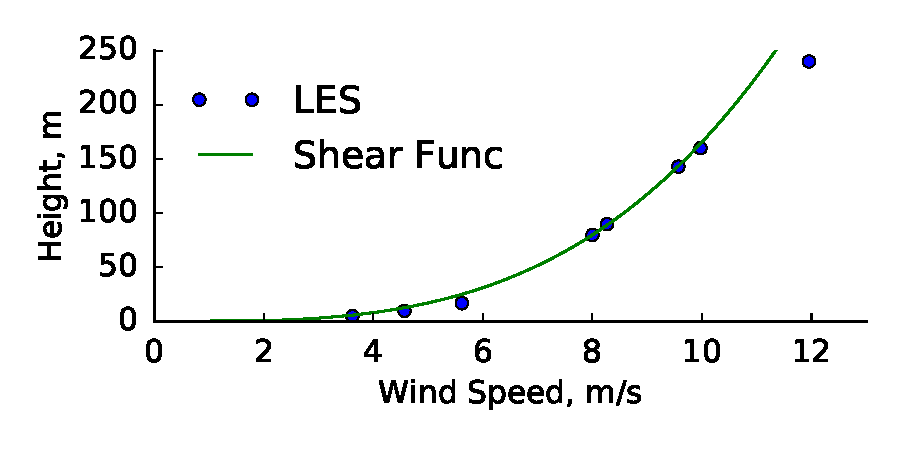
\includegraphics[width=0.5\textwidth]{final_images/shear_fit.pdf}
	\caption{The calculated wind speed using the power law (\Cref{eq:shear}) with shear exponent $\psi=0.31$ compared with the values obtained from the LES precursor. The reference values used were a height of 80 m with a wind speed of 8 m/s.}
	\label{fig:shear_fit}
\end{figure}
%

The discontinuity mentioned previously can occur for various combinations of $k_y$, $k_z$, and $(x-x_0)$. When local turbulence intensity is calculated in the NP wind farm model, as in \cite{niayifar2016} (discussed further in \Cref{sec:npa}), the values of $k_y$ and $k_z$ vary and so the discontinuity is even more mobile than in the original model. We can determine where the model is undefined as follows. First, we know the model is undefined when the condition in \Cref{eq:gt1} is met.
%
\begin{equation}\label{eq:gt1}
	\frac{C_T \cos{\gamma}}{8\sigma_y \sigma_z/d^2} > 1
\end{equation}
%
By substituting \Cref{eq:sigmay,eq:sigmaz} into \Cref{eq:gt1}, and separating the terms based on the powers of $[x-x_0]$, we obtain \Cref{eq:xd1}.
%
\begin{equation}\label{eq:xd1}
	k_y k_z [x-x_0]^2 + \frac{d[k_y+k_z \cos{\gamma}]}{\sqrt{8}}[x-x_0] - \frac{d^2 \cos{\gamma}[C_T -1]}{8} < 0
\end{equation}
%
To find the exact downstream location where the model begins to be defined, $x_d$, we apply the quadratic formula to \Cref{eq:xd1}, select the relevant root, and then solve for $x$ to obtain \Cref{eq:xd}.
%
\begin{equation}\label{eq:xd}
	x_d = x_0 + \frac{d\Bigg[k_y+k_z\cos{\gamma} - \sqrt{[k_y+k_z\cos{\gamma}]^2-4k_y k_z[C_T-1]\cos{\gamma}}\Bigg]}{2k_y k_z\sqrt{8}}
\end{equation}
%
The model, then, is undefined for regions where $x<x_d$. 

To remove the discontinuity, we used linear interpolation on both the velocity value and the wake spread. First, the magnitude of the Gaussian curve at $x_d$ was calculated, as in \Cref{eq:gauss-mag}.
%
\begin{equation}\label{eq:gauss-mag}
	\Delta U_{d_m} = 1 - \sqrt{1 - \frac{C_T \cos{\gamma}}{8 \sigma_{y_d}  \sigma_{z_d}/d^2}}
\end{equation}
%
In \Cref{eq:gauss-mag}, $\sigma_{y_d}$ and $\sigma_{z_d}$ represent the wake spread at $x_d$. Then, using the magnitude of the Gaussian curve, and keeping the wake spread constant for the velocity calculation, the normalized velocity difference is calculated as a function of the downstream position of the point of interest ($x$), as shown in \Cref{eq:bplinear}.
\begin{equation}\label{eq:bplinear}
	\frac{\Delta u_{ij}}{\bar{u}_{i}} = \bigg[x\bigg[\frac{\Delta U_{d_m} - \Delta U_r}{x_d}\bigg] + \Delta U_r\bigg]
        \exp{\bigg(-0.5\bigg[\frac{y-\delta}{ \sigma_{y_d}}\bigg]^2\bigg)}\exp{\bigg(-0.5\bigg[\frac{z-z_h}{ \sigma_{z_d}}\bigg]^2~\bigg)}
\end{equation}
%
In \Cref{eq:bplinear}, $\Delta U_r$ is a predetermined normalized velocity deficit at the rotor hub. To avoid overpredicting the velocity deficits and potentially causing an unrealistic flow reversal,  we used a value of $\Delta U_r=\Delta U_{d_m}$. 

The results of the model changes discussed above are shown in \Cref{fig:model_contours}. These changes make the model continuous throughout the domain and differentiable everywhere except at the exact turbine location. With a separation constraint in place, the probability of turbines landing exactly on top of each other is extremely small, as noted in \cite{thomas2017}. With the linear interpolation method, optimizations succeed even when turbines are placed less than 1 diameter from each other. While the linear interpolation makes little attempt to be physically accurate in the near-wake, the accuracy of the model for AEP calculation purposes should be unaffected since turbines will almost never be placed close enough together to be in the linear interpolation region in a final design. If greater accuracy is desired in the near-wake, it would be feasible to use the linear interpolation during optimization and then switch to a more accurate near-wake model for final calculations, such as the one proposed in \cite{keane2016}.

\begin{figure}[htbp!]
	\centering
	\subfigure[]{
		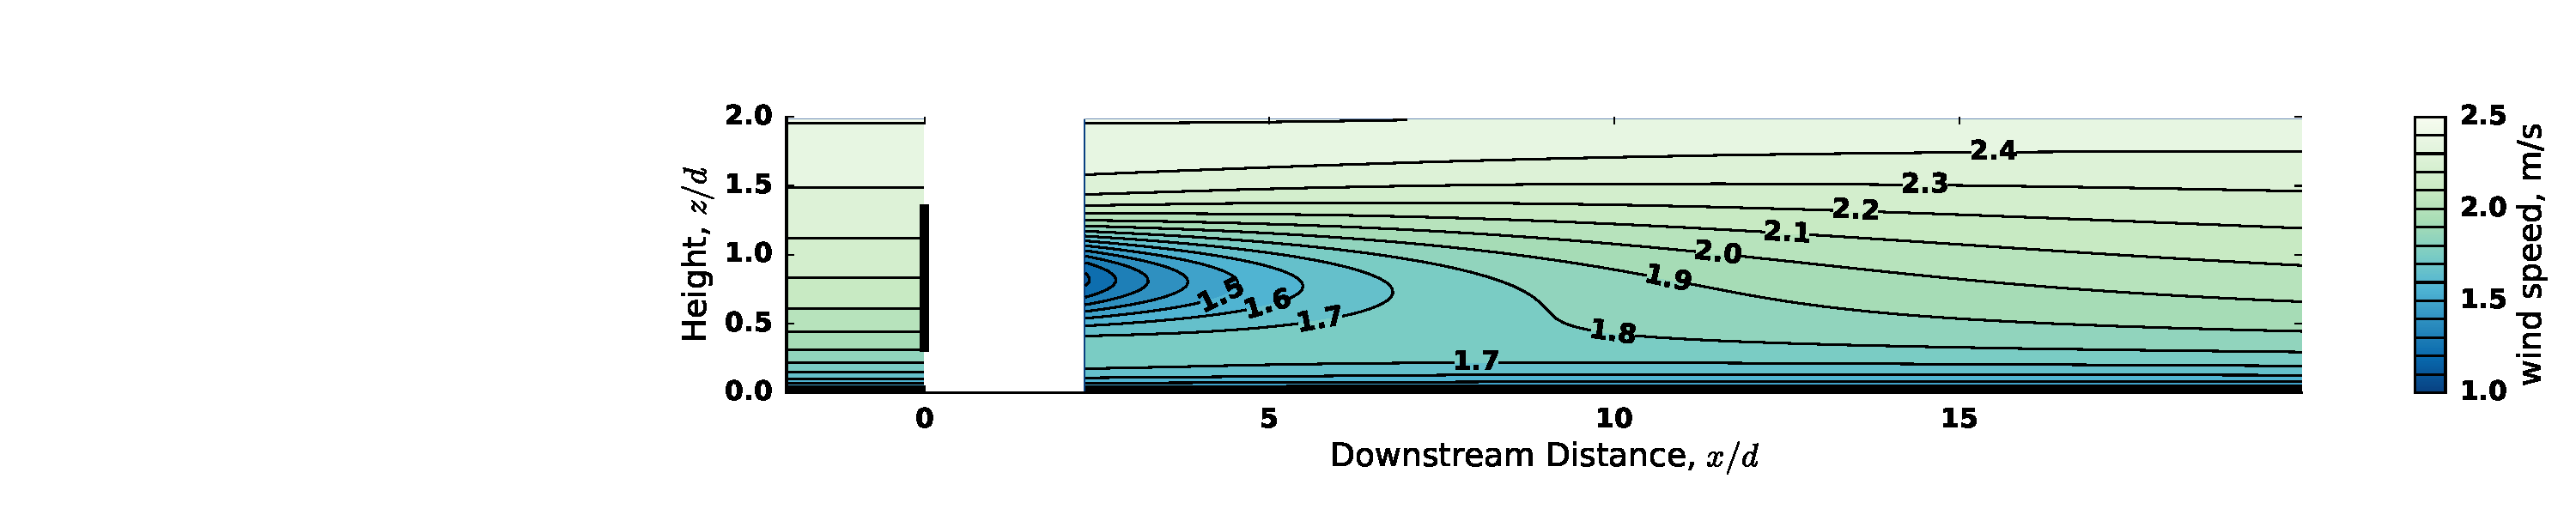
\includegraphics[width=0.75\textwidth, trim={18.5cm 1cm 4.cm 1cm}]{final_images/model_contours_vertical_before.pdf}
	}
	\subfigure[]{
		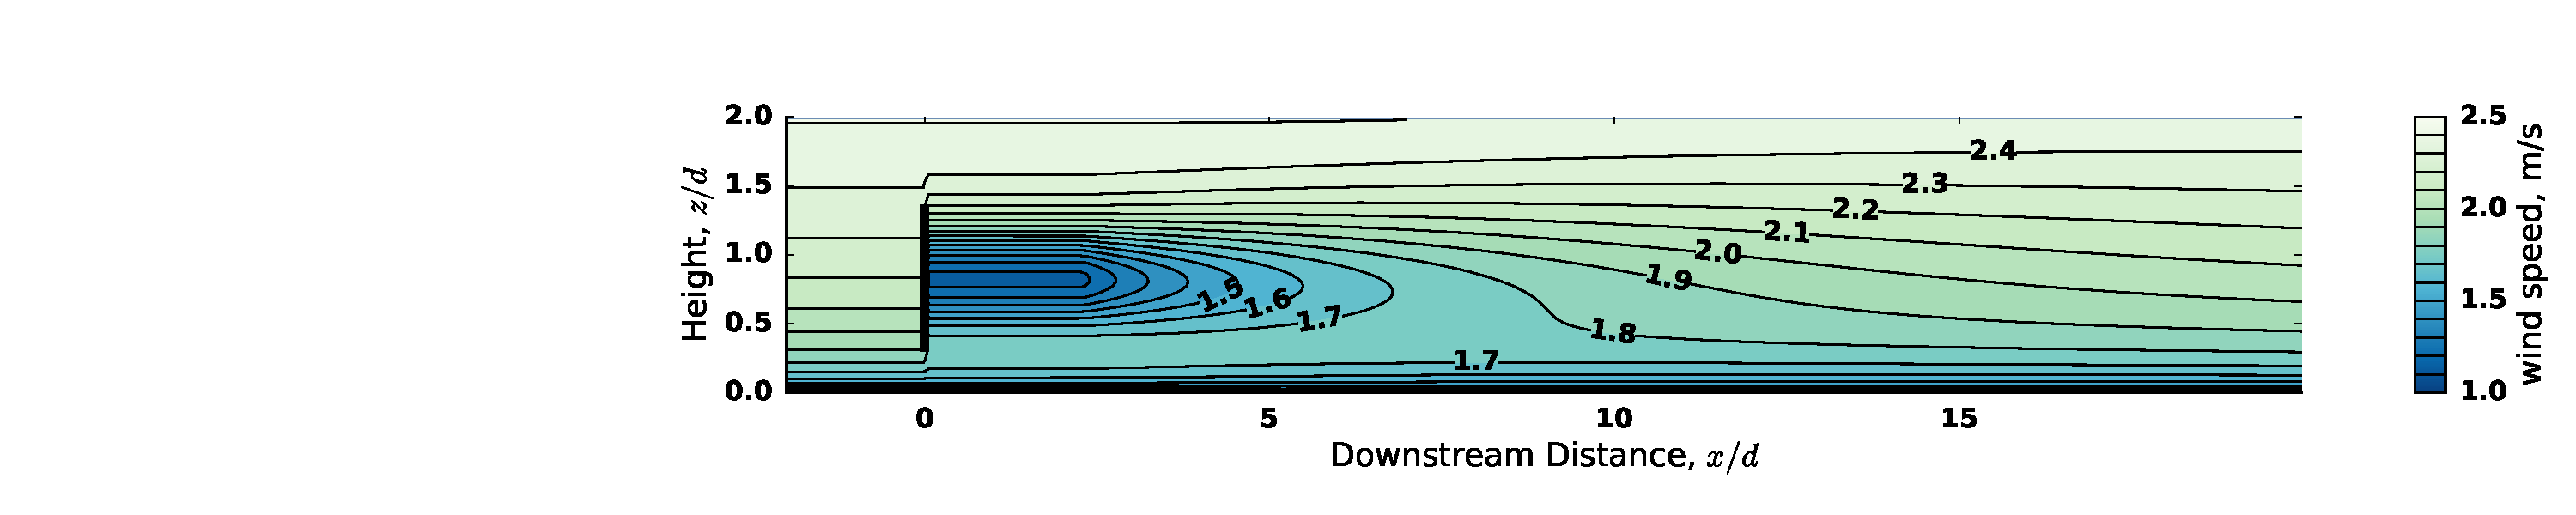
\includegraphics[width=0.75\textwidth, trim={18.5cm 1cm 4.cm 1cm}]{final_images/model_contours_vertical_after.pdf}
	}
	\caption{Bastankhah and Port\'{e}-Agel wake model (a) without and (b) with the added linear interpolation for the near-wake. The heavy black line represents the turbine rotor. This figure was included for comparison with Fig. 6 of Bastankhah and Port\'{e}-Agel (2014) \cite{bastankhah2014}, and so model values were chosen accordingly (small wind turbine for use in a wind tunnel). We used a shear exponent of 0.15 for this figure.}
	
	\label{fig:model_contours}
\end{figure}

\subsection{Wind Farm Model}\label{sec:npa}
NP proposed a wind farm model that used the BP model as published in 2014 \cite{bastankhah2014} for calculating the wind speed in the wakes \cite{niayifar2015, niayifar2016}. We applied the same wind farm model to the 2016 version of the BP model, with some variation as discussed in the following sections.
% However, due to changes made to the Bastankhah and Port\'{e}-Agel wake model published in 2016 \cite{bastankhah2016}, along with the needs of gradient-based optimization, not all of the proposals made by Niayifar and Port\'{e}-Agel in their 2016 paper can be used. This section will discuss which aspects of the Niayifar and Port\'{e}-Agel model that were and were not used in our system.
\subsubsection{Wake Combination}
NP found the most accurate method of wake combination to be a linear velocity deficit superposition that uses the inflow velocity of the upstream turbine as shown in \Cref{eq:wake-comb-lin}. 
%
\begin{equation}\label{eq:wake-comb-lin}
	u_j = \bar{u}_\infty - \sum_{i=1}^{N_T} [\bar{u}_i - u_{ij}] = \bar{u}_\infty - \sum_{i=1}^{N_T} \Delta u_{ij}
\end{equation}
%
In \Cref{eq:wake-comb-lin}, $u_j$ is the flow velocity at the point of interest, $\bar{u_i}$ is the average inflow velocity of upstream turbine $i$, $u_{ij}$ is the wind speed that would exist at the point $j$ if only turbine $i$ were accounted for, and $\bar{u}_{\infty}$ is the average free-stream velocity. For the upstream turbine velocity to be used, the inflow velocity of the turbines must be calculated in order from upstream to downstream. We used the heapsort algorithm to obtain a sorted index list of the turbines prior to solving the system for each wind direction. Using the sorted index list allowed turbine sorting without overcomplicating the gradients of the system. Our tests of the accuracy of various wake combination methods also found this method to be the most accurate in comparison to the LES results used by Niayifar and Port\'{e}-Agel in \cite{niayifar2016}.

\subsubsection{Turbulence Intensity}\label{sec:ti}
Niayifar and Port\'{e}-Agel calculated local turbulence intensity using the model presented by Crespo and Hern\'{a}ndez in \cite{crespo1996}. The local turbulence intensity is then applied to the BP model through an empirical model for calculating the wake expansion coefficient as shown in \Cref{eq:ti_npa} \cite{niayifar2016}.
 %
 \begin{equation} \label{eq:ti_npa}
 	k^* = 0.3837 I + 0.003678
 \end{equation}
%
In \Cref{eq:ti_npa}, $I$ is the turbulence intensity (TI). This model is only valid for TI values between 0.065 and 0.15. While the initial BP wake model does not include TI \cite{bastankhah2014}, TI was included by Bastankhah and Port\'{e}-Agel in their 2016 version of the model \cite{bastankhah2016}. We used the same TI values for the BP 2016 wake model and the NP wind farm model. 

The algorithm for calculating local turbulence intensity using the hard maximum function is given in \Cref{alg:ti}. In our code implementation, we combined the nested loops used for the velocity and TI calculations. 
%
\begin{algorithm}[htpb!]
	\caption{Turbulence Intensity Calculation (for more information, see \cite{niayifar2016})}
   \label{alg:ti}
   \begin{algorithmic}
   \Ensure Turbines are sorted by relative downstream position
     \For{$j =  1...N$} \Comment{Downstream turbines}
   	% \State $I_j \gets I_0$ \Comment{Initialize to free-stream turbulence value}
    \State $A_{r_j} \gets \frac{1}{4}\pi D_{r_j}^2$ \Comment{Rotor swept area of turbine $j$}
    \State $I_{+_j} \gets 0$
         \For{$i =  1...N$} \Comment{Upstream turbines}
         	\State $\Delta X \gets x_j - x_i$ \Comment{Turbine separation distance}
         	\If{$\Delta X > 0$}
               \State $\beta \gets 0.5\Big[\Big[1+\sqrt{1-C_{T_i}}\Big]/\sqrt{1-C_{T_i}}\Big]$
               \State $\epsilon \gets 0.2 \sqrt{\beta}$
               \State $\sigma = k_i^*\Delta X+D_{r_i}\epsilon$
               \State $D_w \gets 4\sigma$
               \State $A_{w_{ij}} \gets$ Wake overlap area of wake $i$ and rotor $j$ \Comment{Assume circular wake}
               \If{$C_{T_i} > 0.96$}
                    \State $a_i \gets 0.143 + \sqrt{0.0203-0.6427[0.889 - C_{T_i}]}$ \Comment{Glauert correction \cite{gebraad2017-max-aep}}
               \Else
                   \State $a_i \gets  \frac{1}{2}\Big[1-\sqrt{1-C_{T_i}}\Big]$
               \EndIf
               
               \State $I_{+_{ij}} \gets 0.73 a_{i}^{0.8325} I_i^{0.0325} [\Delta X/D_{r_i}]^{-0.32}$
               \State $I_{+_j} \gets \max{[I_{+_{ij}}A_{w_{ij}}/A_{r_j}, I_{+_j}]}$ \Comment{We used \Cref{eq:smoothmax3} during the final optimization}
        	\EndIf
        \EndFor
        \State $I_j \gets \sqrt{I_{0}^2 + I_{+_j}^2}$ \Comment{Directly influenced by only one upstream turbine}
        \State $k_j^* \gets 0.3837I_j+0.003678 $ \Comment{To be used in the wake model calculations}
     \EndFor
   \end{algorithmic}    
\end{algorithm}
%

We used three different approaches to calculating TI at various points in the optimization process: (1) ambient TI only, (2) local TI with a smooth maximum function, and (3) local TI with a hard maximum function as done by Niayifar and Port\'{e}-Agel \cite{niayifar2016} and shown in \Cref{alg:ti}. The reasons for using the three methods for calculating TI are discussed in \Cref{sec:opt}. The smooth maximum function we used is shown in \Cref{eq:smoothmax1,eq:smoothmax2,eq:smoothmax3} and is derived from the LogSumExp function \cite{cook2010-softmaximum}.
%
\begin{equation}\label{eq:smoothmax1}
    t_{max} = \min(t_1, t_2)
\end{equation}
\begin{equation}\label{eq:smoothmax2}
    t_{min} = \max(t_1, t_2)
\end{equation}
\begin{equation}\label{eq:smoothmax3}
  \text{max}_{smooth}(t_{max},t_{min},s) = \frac{\ln(1+\exp(s[t_{min}-t_{max}]))+s t_{max}}{s}
\end{equation}
%
In \Cref{eq:smoothmax1,eq:smoothmax2,eq:smoothmax3}, $s$ controls the smoothness of the transition between terms and influences the error of the calculation and $t_{max}$ and $t_{min}$ represent the respective maximum and minimum of the two values being compared. In calculating local turbulence intensity, \Cref{eq:smoothmax3} is applied, as in  \Cref{eq:maxti}, to compare the product of the added local turbulence intensity and the wake overlap ratio.
%
\begin{equation}\label{eq:maxti}
    I_{+_j} = \text{max}_{smooth}{\bigg(\frac{I_{+_{ij}}A_{w_{ij}}}{A_{r_j}}\bigg)}
\end{equation}
%
In \Cref{eq:maxti}, $A_{w_{ij}}$ is the area of the wake of turbine $i$ at the downstream location of turbine $j$, $A_{r_j}$ is the area of the rotor of turbine $j$, and $I_{+_{ij}}$ is the added turbulence intensity from turbine $i$ at the downstream location of turbine $j$. In our implementation, only two values are compared at a time; the current value and the previous result of the smooth maximum function. The total turbulence intensity is then calculated using \Cref{eq:ti_at_turb}.
%
\begin{equation}\label{eq:ti_at_turb}
    I_j = \sqrt{I_0^2+I_{+_j}^2}
\end{equation}
%
The maximum error of \Cref{eq:smoothmax3} occurs when $t_{min} = t_{max}$, and can be calculated as in \Cref{eq:error_max}.
%
\begin{equation}\label{eq:error_max}
	\text{Error}_{max} = \frac{\ln{(2)}}{s}
\end{equation}
%
To keep the error from the smooth maximum below 0.001, or about 1\% of the total turbulence intensity, we set $s=700$.

% Using \Cref{eq:ti_npa} in the updated wake model would cause the effects of turbulence intensity to be included twice. We used \Cref{eq:ti_npa} to estimate the initial $k^*$ only. Within the model itself, the ambient turbulence intensity only impacts the model through Bastankhah and Port\'{e}-Agel (2016) \cite{bastankhah2016} and local turbulence intensity is not calculated. 
%
%Jen changes
% \begin{algorithm}
% 	\caption{Turbulence Intensity Calculation}
%    \label{alg:ti}
%    \begin{algorithmic}
%    \Ensure Turbines are sorted by relative downstream position
%      \For{$j =  1...N$} \Comment{Downstream turbines}
%    	\State $I_{+,j} \gets 0$
%          \For{$i =  1...N$} \Comment{Upstream turbines}
%          	\State $\Delta X \gets x_j - x_i$ 
%          	\If{$\Delta X > 0$}
%                \State $\beta \gets 0.5((1+\sqrt{1-C_{T,i}})/\sqrt{1-C_{T,i}})$
%                \State $\epsilon \gets 0.2 \sqrt{\beta}$
%                \State $\sigma = k_i^*\Delta X+D_{r,i}\epsilon$
%                \State $D_w \gets 4\sigma$
%                \State $A_{w,i,j} \gets$ Wake overlap area of wake $i$ and rotor $j$ \Comment{Circular wake}
%                \State $A_{r,j} \gets \pi D_{r,j}^2/4$ \Comment{Rotor-swept area}
%                \State $I_{+,i,j} \gets 0.73 a_{i}^{0.8325} I_{0,i}^{0.0325} (\Delta X/D_{r,i})^{-0.32}$
%                \State $I_{+,j} \gets \max{((I_{+,i,j}A_{w,i,j}/A_{r,j}), (I_{+,i-1}))}$ \Comment{Discontinuity here}
%         	\EndIf
%         \EndFor
%         \State $I_{0,j} \gets \sqrt{I^2 + I_{+,j}^2}$
%         \State $k_j^* \gets 0.3837I_{0,j}+0.003678 $ \Comment{To be used in the BPA wake model}
%      \EndFor
%    \end{algorithmic}    
% \end{algorithm}
% 

\subsubsection{Sampling Over the Rotor-Swept Area}
Various methods can be used to approximate the effective velocity at the rotor. The ideal method is a full integration across the rotor-swept area. We approximated the integral by sampling the velocity at various points and taking the average. 
%Maximum and average directional error, as compared to the directional power LES results from \cite{niayifar2016}, is shown in \cref{fig:sampling-error}. 
%\begin{figure}[ht]
%	\centering
%	\subfigure[]{
%		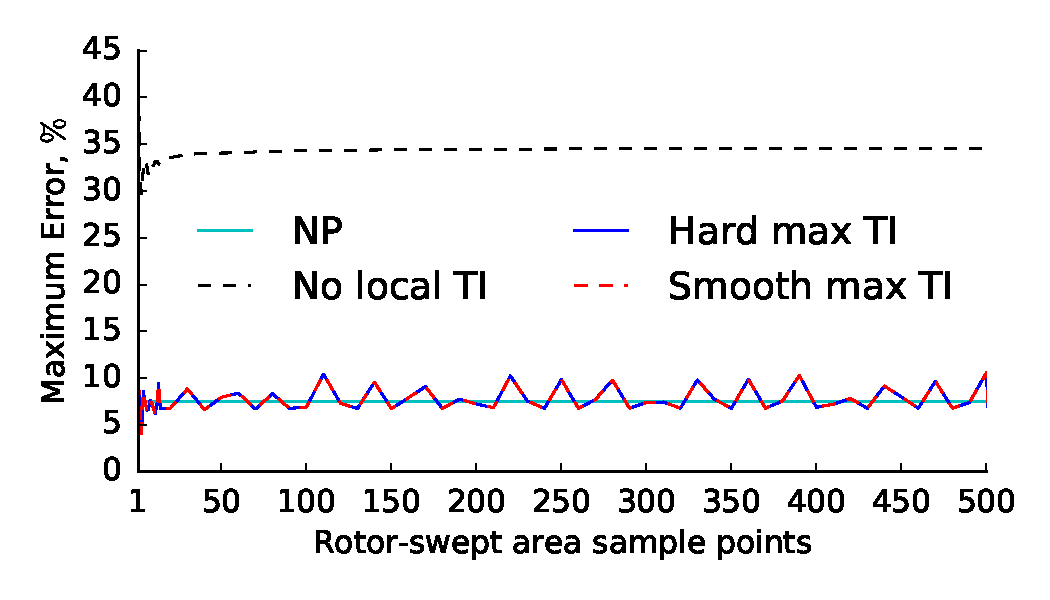
\includegraphics[width=0.48\textwidth, trim={0cm 0cm 0cm 0cm}]{final_images/power_by_dir_vs_rpts_max_error.pdf}
%	}
%    \subfigure[]{
%		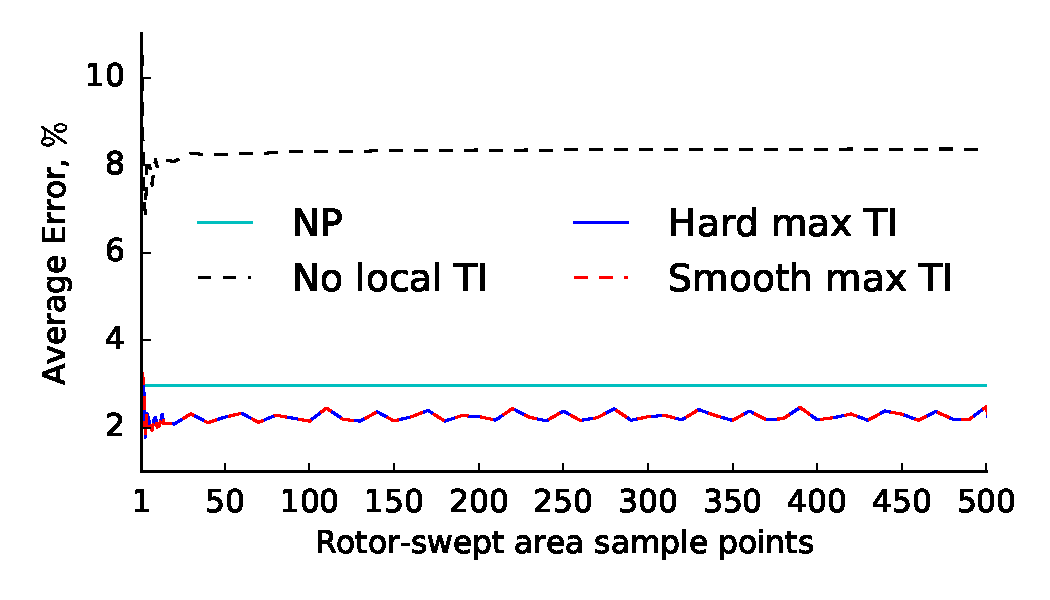
\includegraphics[width=0.48\textwidth, trim={0cm 0cm 0cm 0cm}]{final_images/power_by_dir_vs_rpts_ave_error.pdf}
%	}
%% 	\subfigure[]{
%% 		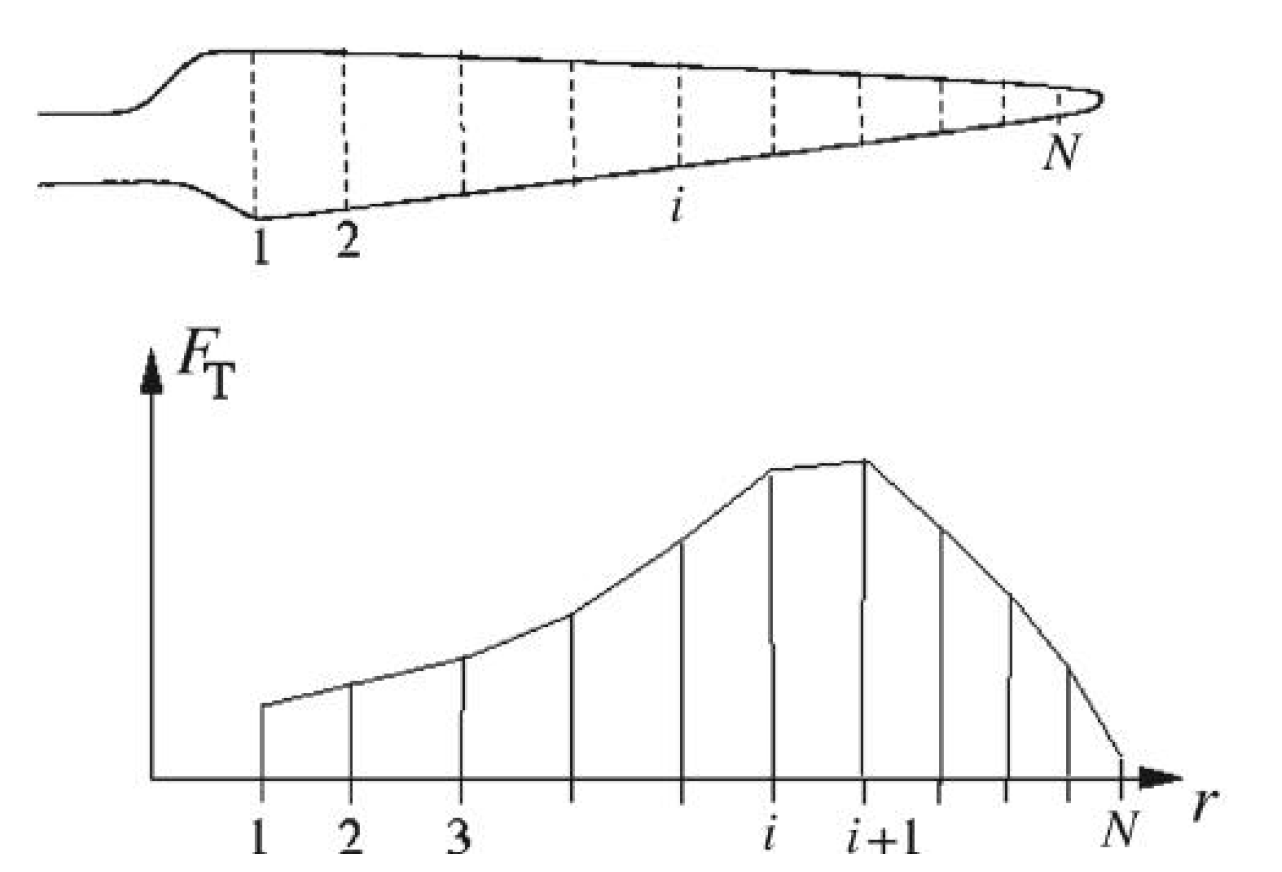
\includegraphics[width=0.43\textwidth, trim={0cm -1cm 0cm 0cm}]{final_images/bem_distribution.png}
%% 	}
%	\caption{Maximum (a) and average (b) directional power production error for varrying numbers of velocity samples on the rotor-swept area using the BP model as compared to LES results for Horns rev from \cite{niayifar2016}.}
%	\label{fig:sampling-error}
%\end{figure}
When comparing our code to LES and other data, we used 100 sampling points across the rotor-swept area arranged in the sunflower seed pattern as shown in \Cref{fig:sampling_locs}(a). We found that 100 sample points on the rotor-swept area were more than sufficient to achieve the level of accuracy demonstrated by Niayifar and Port\'{e}-Agel in \cite{niayifar2016}. For efficiency during optimization, we approximated the effective velocity of each wind turbine by using a single sampling point located at the rotor hub as shown in \Cref{fig:sampling_locs}(b).

\begin{figure}[ht]
	\centering
	\subfigure[]{
		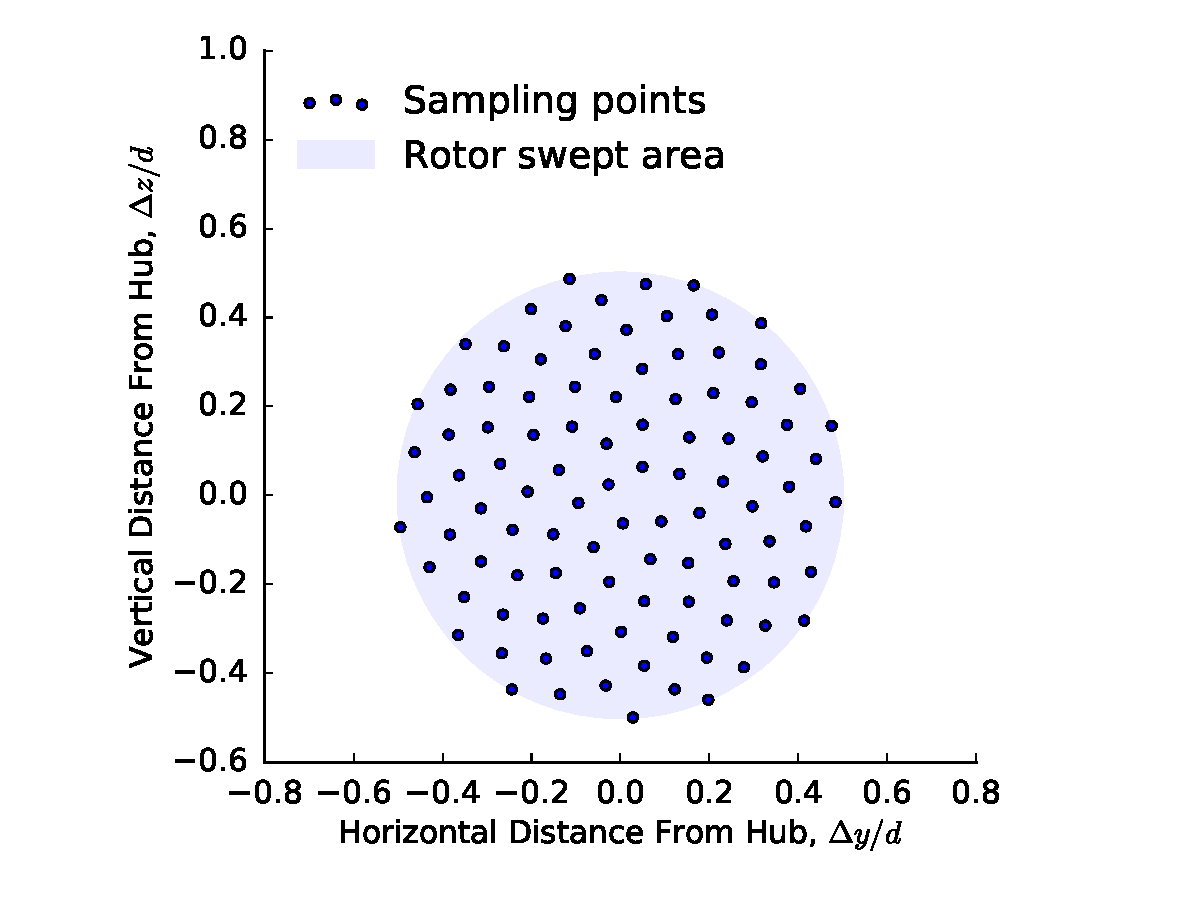
\includegraphics[width=0.48\textwidth, trim={0cm 0cm 0cm 0cm}]{final_images/one_hundred_sampling_points.pdf}
	}
    \subfigure[]{
		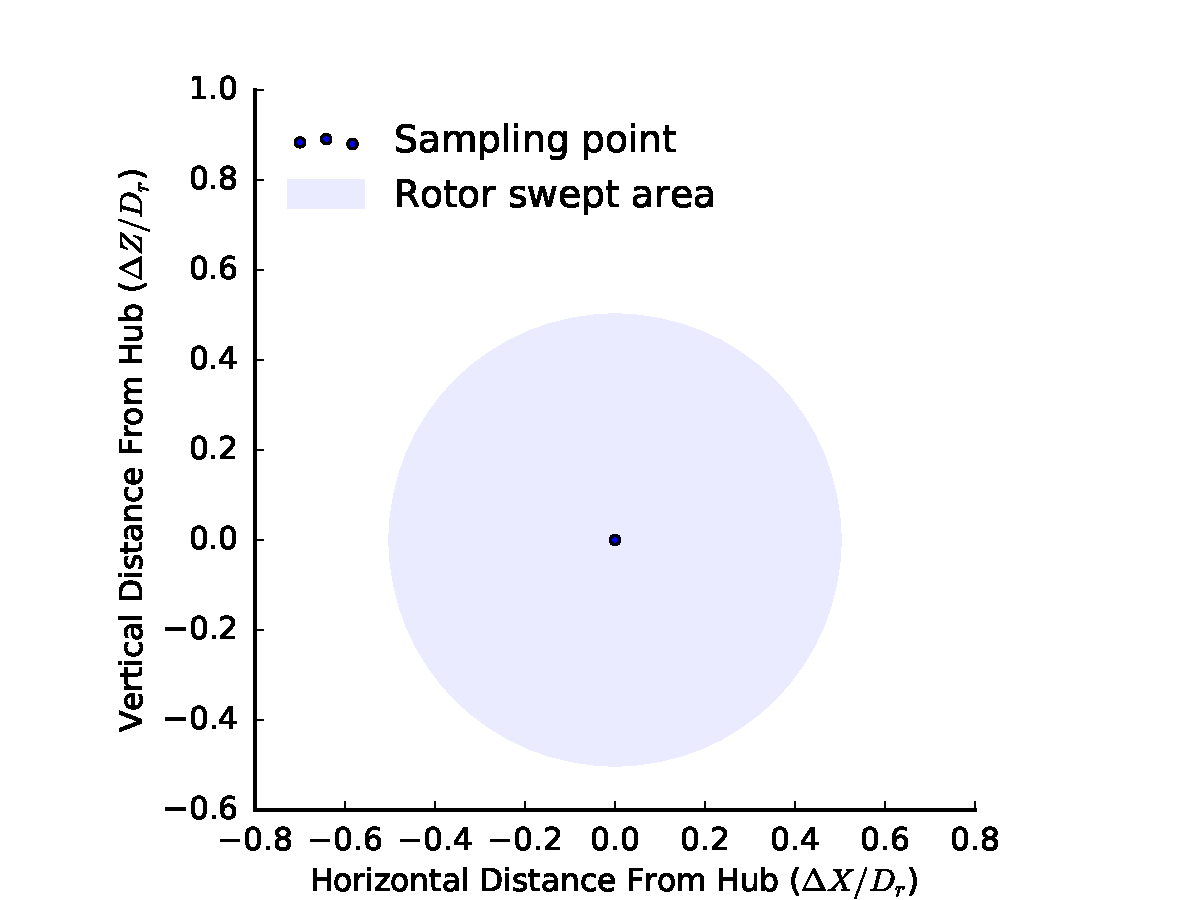
\includegraphics[width=0.48\textwidth, trim={0cm 0cm 0cm 0cm}]{final_images/one_sampling_point.pdf}
	}
% 	\subfigure[]{
% 		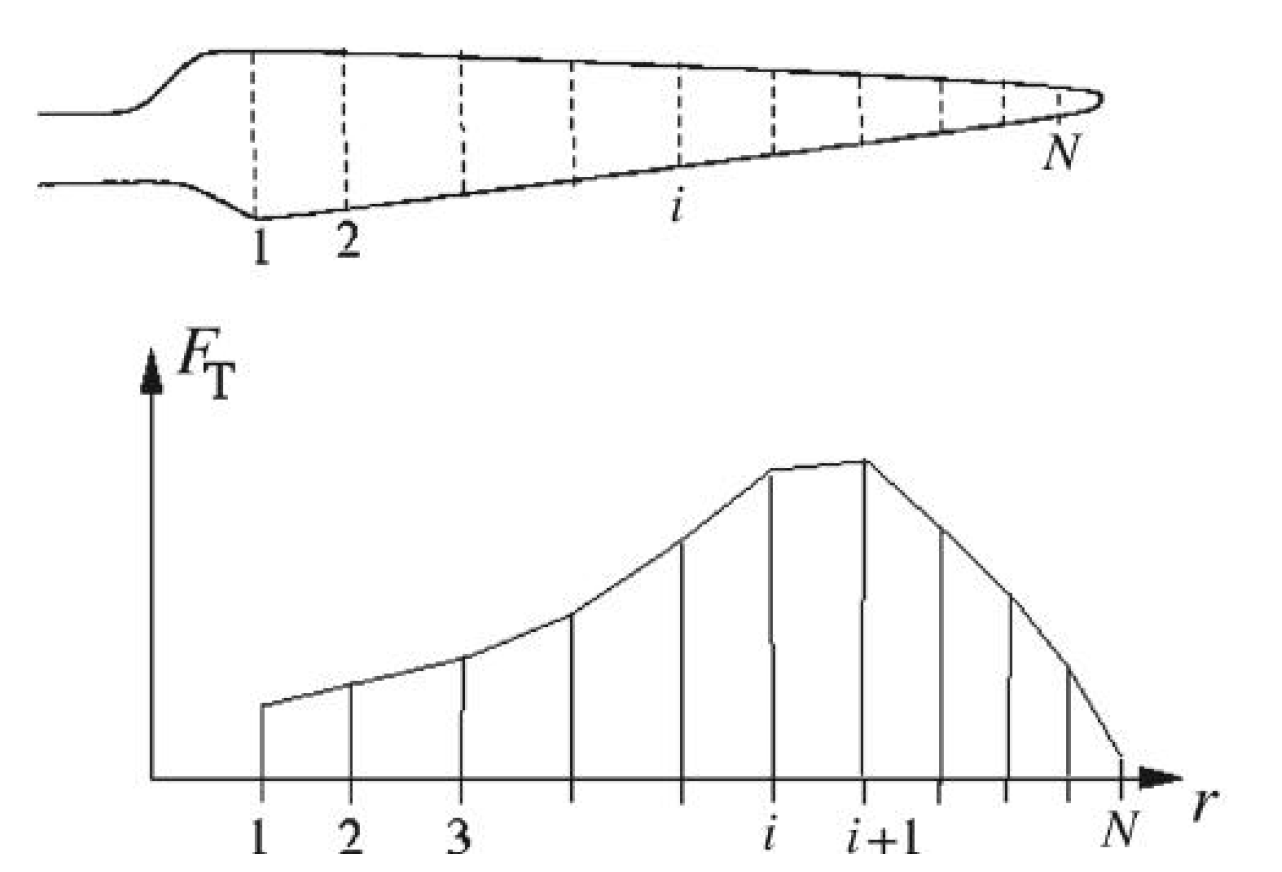
\includegraphics[width=0.43\textwidth, trim={0cm -1cm 0cm 0cm}]{final_images/bem_distribution.png}
% 	}
	\caption{(a) Sampling locations used to approximate effective hub velocity for LES comparisons. (b) Location of sampling point for approximating effective hub velocity during optimization.}
	\label{fig:sampling_locs}
\end{figure}

\subsubsection{AEP and Wind Turbine Power}
AEP was calculated as in \Cref{eq:aep}.
\begin{equation}
    \label{eq:aep}
    AEP = \bigg[\frac{hours}{day}\bigg]\bigg[\frac{days}{year} \bigg]\sum_{k=1}^{N_D} \bigg[ f_k \sum_{j=1}^{N_T}P_{j_k} \bigg]
\end{equation}
%
In \Cref{eq:aep}, $N_D$ is the number of wind directions, $N_T$ is the number of wind turbines, and $f_k$ is the probability of wind in direction $k$. The power of turbine $j$ in direction $k$, $P_{j_k}$, is calculated based on the definition of the power coefficient as done in \cite{gebraad2014} and shown in \Cref{eq:power}.
%
\begin{equation}\label{eq:power}
    P_{j_k} = 
    \begin{cases} 
      0 & \bar{u}_j < u_{cutin} \\
      0.5\rho A_j C_{P_j}\bar{u}_j^3 & \bar{u}_j \geq  u_{cutin} \ \text{and} \ P_{j} < P_{rated} \\
      P_{rated} & P_{j} \geq P_{rated}
\end{cases}
\end{equation}
%
In \Cref{eq:power}, $\rho$ is the air density, $A_j$ represents the rotor-swept area of turbine $j$, and $C_{P_j}$ is the power coefficient of turbine $j$ for the given effective wind speed at the rotor ($\bar{u}_j$).

\subsubsection{Model Verification}
To verify our implementation of the models described, we compared the output of our code with data for the Horns Rev wind farm from Niayifar and Port\'{e}-Agel \cite{niayifar2016} as shown in \Cref{fig:power_line,fig:power_direction}. We calculated error, in normalized power, based on the LES data values from \cite{niayifar2016} and reported the error in \Cref{tab:validation-error}. For the Horns Rev row-averaging comparison using 100 samples on the rotor-swept area as shown in \Cref{fig:power_line}(a): the model values shown by Niayifar and Port\'{e}-Agel had an average error of $0.034$ and a maximum error of $0.057$; ignoring local turbulence intensity resulted in an average error of $0.179$ and a maximum error of $0.253$; calculating local turbulence intensity using either the hard maximum or smooth maximum both resulted in an average error of $0.018$ and a maximum error of $0.035$.  For the Horns Rev directional power comparison using 100 samples on the rotor-swept area as shown in \Cref{fig:power_direction}(a): the model values shown by Niayifar and Port\'{e}-Agel had an average error of $0.022$ and a maximum error of $0.055$; ignoring local turbulence intensity resulted in an average error of $0.058$ and a maximum error of $0.206$; calculating local turbulence intensity using either the hard maximum or smooth maximum both resulted in an average error of $0.017$ and a maximum error of $0.053$. The high directional errors when local turbulence intensity is ignored are in the directions of highest wake interactions as shown in \Cref{fig:power_direction} and do not alter the general trend of the directional power. The Horns Rev comparisons using one sample on the rotor-swept area are shown in \Cref{fig:power_line}(b) and \Cref{fig:power_direction}(b). Using only one sample on the rotor-swept area resulted in slightly larger errors as reported in \Cref{tab:validation-error}. Based on our model error being within the range reported in \cite{niayifar2016} when we used 100 samples and local TI (less than $0.057$ and $0.055$ for the row and directional comparisons, respectively), we determined that our implementation of the BP wake and NP farm models was sufficient and could be used to perform wind farm layout optimization case studies.

\begin{figure}[htbp!]
	\centering
	\subfigure[]{
		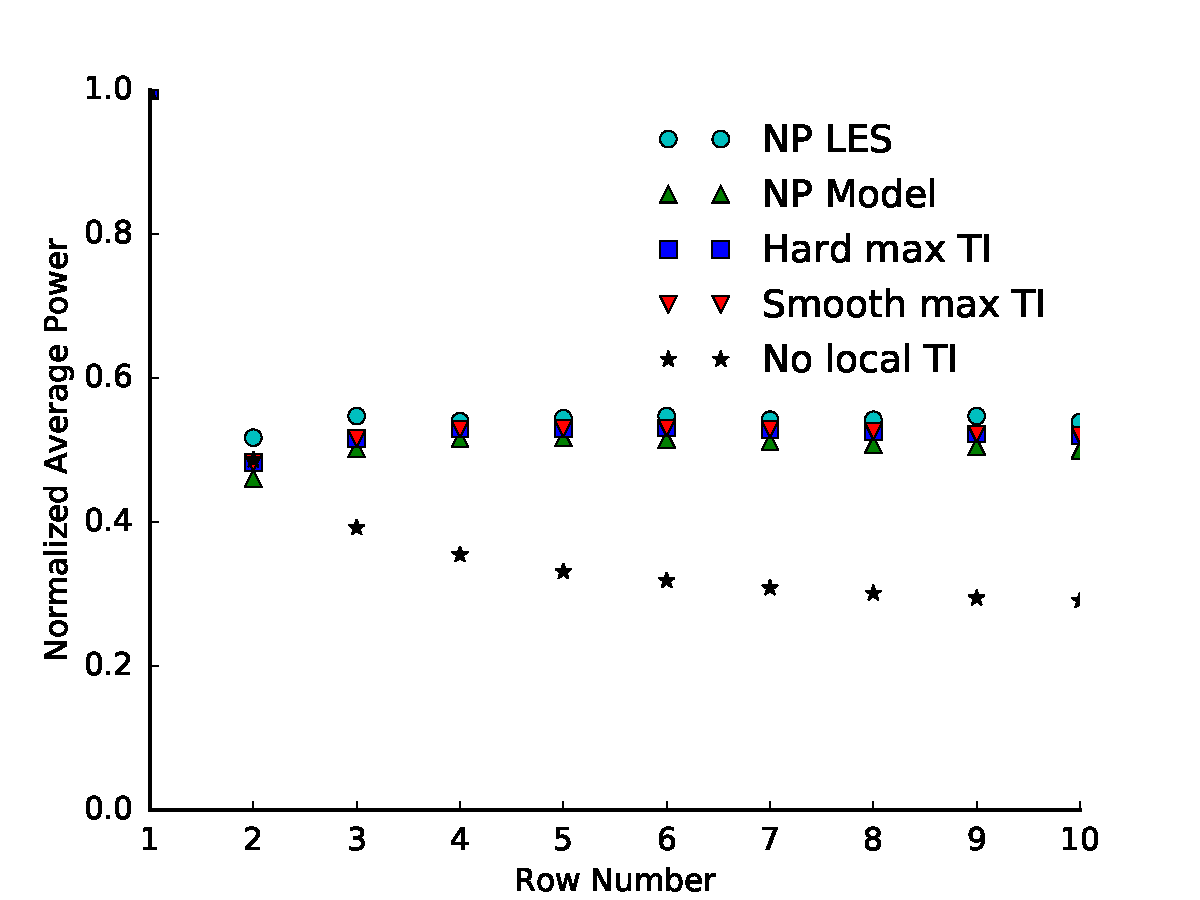
\includegraphics[width=0.48\textwidth, trim={0cm 0cm 0cm 0cm}]{final_images/power_by_row_horns_rev_100rpt.pdf}
	}
	\subfigure[]{
		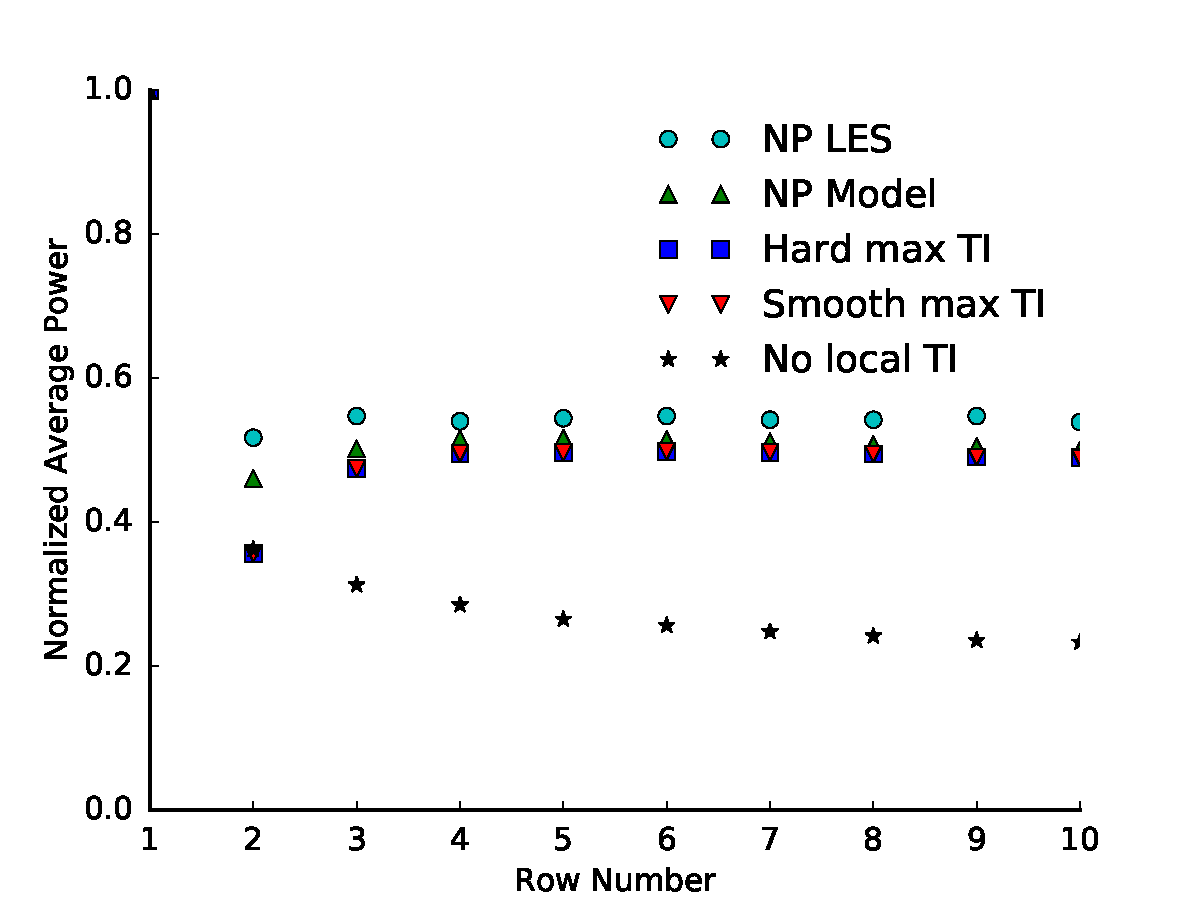
\includegraphics[width=0.48\textwidth, trim={0cm 0cm 0cm 0cm}]{final_images/power_by_row_horns_rev_1rpt.pdf}
	}
	\caption{Averaged power of turbines in columns two, three, and four of the Horns Rev wind farm by turbine row. (a) Comparing our code using 100 points to approximate the effective wind speed at the rotor. (b) Comparing our code using a single sample at the rotor hub to approximate the effective wind speed at the rotor. NP refers to LES and model results from \cite{niayifar2016}. All three methods of calculating TI refer to results obtained using our code. The three methods for calculating TI are to address various complications during our optimization process (see \Cref{sec:ti,sec:opt} for details).}
	\label{fig:power_line}
\end{figure}

\begin{figure}[htbp!]
	\centering
	\subfigure[]{
		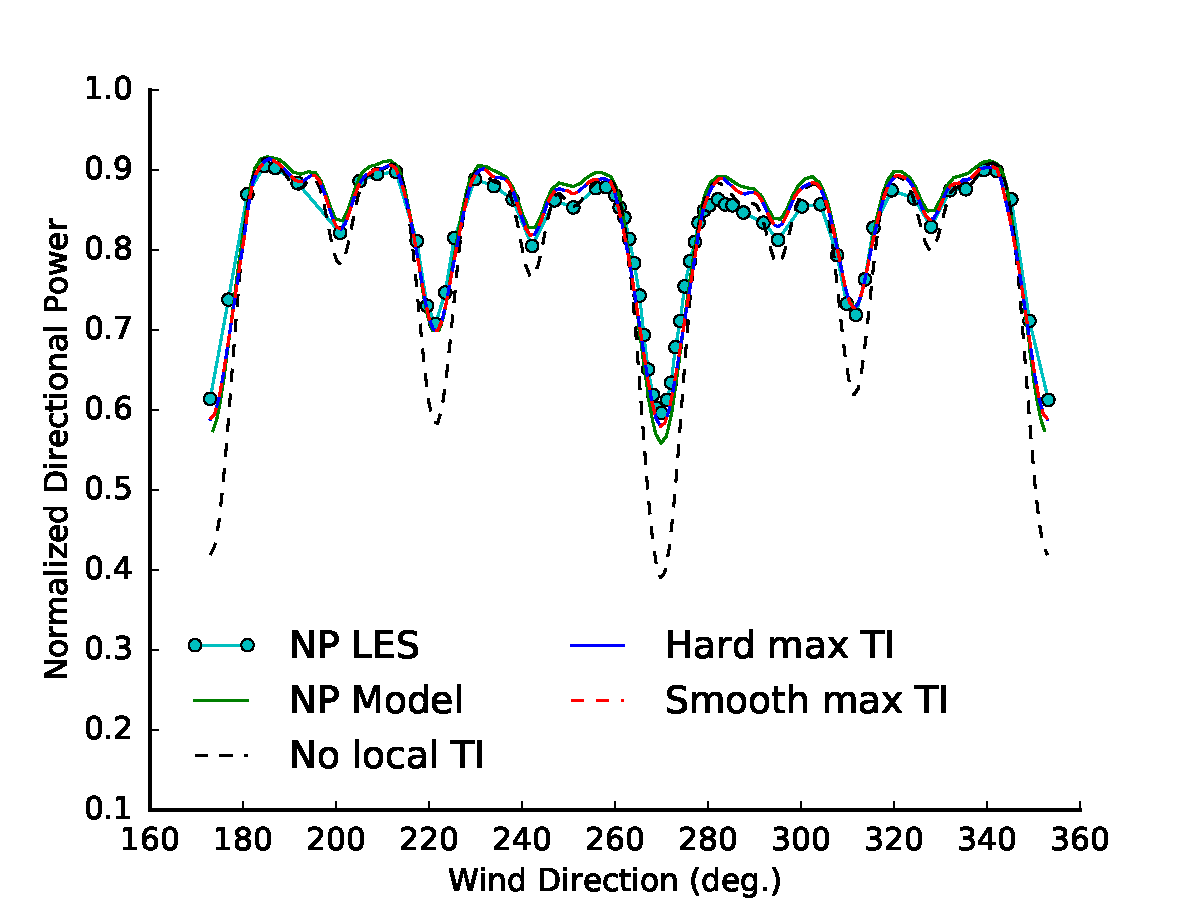
\includegraphics[width=0.48\textwidth, trim={0cm 0cm 0cm 0cm}]{final_images/power_by_dir_horns_rev_100rpt.pdf}
	}
	\subfigure[]{
		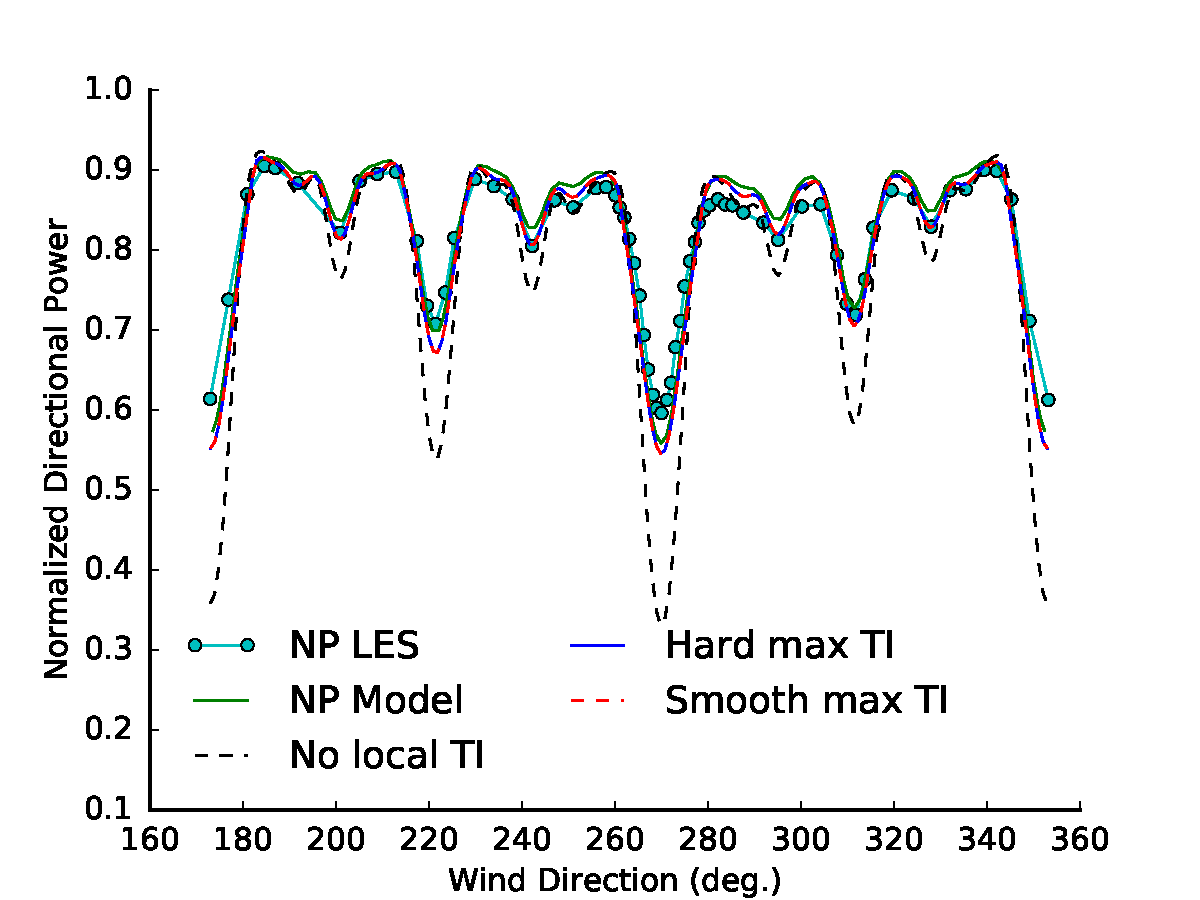
\includegraphics[width=0.48\textwidth, trim={0cm 0cm 0cm 0cm}]{final_images/power_by_dir_horns_rev_1rpt.pdf}
	}
	\caption{Power by direction for the Horns Rev wind farm. (a) Comparing our code using 100 points to approximate the effective wind speed at the rotor. (b) Comparing our code using a single sample at the rotor hub to approximate the effective wind speed at the rotor. NP refers to LES and model results from \cite{niayifar2016}. All three methods of calculating TI refer to results obtained using our code. The three methods for calculating TI are to address various complications during our optimization process (see \Cref{sec:ti,sec:opt} for details).}
	
	\label{fig:power_direction}
\end{figure}

\begin{table*}[htpb!]\centering
\caption{Normalized model power error as compared to Horn Rev LES results \cite{niayifar2016}.}\label{tab:validation-error}
\ra{1.3}
\begin{tabular}{@{}llrcrrcrrcrr@{}}\toprule
& & & & \multicolumn{2}{c}{No Local TI} &\phantom{a}& \multicolumn{2}{c}{Hard Max TI} &\phantom{a}& \multicolumn{2}{c}{Smooth Max TI}\\ 
\cmidrule{5-6} \cmidrule{8-9} \cmidrule{11-12}

& &  &  \phantom{a} & \multicolumn{2}{c}{Samples} & \phantom{a}&\multicolumn{2}{c}{Samples} & \phantom{a}&\multicolumn{2}{c}{Samples}\\ 
% \cmidrule{5-6} \cmidrule{8-9} \cmidrule{11-12}

& & \multicolumn{1}{c}{NP Model} & \phantom{a} & \multicolumn{1}{c}{100} & \multicolumn{1}{c}{1} & \phantom{a} &\multicolumn{1}{c}{100} & \multicolumn{1}{c}{1} & \phantom{a} & \multicolumn{1}{c}{100} & \multicolumn{1}{c}{1} \\ 
 \cmidrule{3-3} \cmidrule{5-6} \cmidrule{8-9} \cmidrule{11-12}

%directional 100 samples
%error for direction horns rev - not percent
%NPA ave error 0.0224456601583
%NPA max error 0.0548174348544
%no ti ave error 0.0580638689657
%no ti max error 0.206232309586
%hard max ave error 0.0167584587067
%hard max max error 0.0525671878498
%smooth max ave error 0.0167580458573
%smooth max max error 0.052567187849

% direcrtional 1 sample
%error for direction horns rev - not percent
%NPA ave error 0.0224456601583
%NPA max error 0.0548174348544
%no ti ave error 0.0738947693338
%no ti max error 0.265977544296
%hard max ave error 0.0248056484519
%hard max max error 0.0721467766148
%smooth max ave error 0.0248023899965
%smooth max max error 0.0721467766137

\multicolumn{1}{c|}{\multirow{2}{*}{Directional}}  &  \multicolumn{1}{l}{Max} &0.055 & & 0.206 &0.266  & & 0.053 &0.072  & & 0.053 & 0.072\\
\multicolumn{1}{c|}{} &  \multicolumn{1}{l}{Average} &0.022  & &0.058 &0.074 & & 0.017 &0.025 & & 0.017 &0.025\\

\\
% line 100 samples
%error for direction horns rev - not percent
%NPA ave error 0.0343720467811
%NPA max error 0.0568312420913
%no ti ave error 0.178899266747
%no ti max error 0.252759908164
%hard max ave error 0.0181504489593
%hard max max error 0.0345533848729
%smooth max ave error 0.0181504489244
%smooth max max error 0.0345533848729

% 1 sample
%error for direction horns rev - not percent
%NPA ave error 0.0343720467811
%NPA max error 0.0568312420913
%no ti ave error 0.242767970086
%no ti max error 0.311590313116
%hard max ave error 0.0575680259789
%hard max max error 0.160582538608
%smooth max ave error 0.0575680259386
%smooth max max error 0.160582538608


\multicolumn{1}{c|}{\multirow{2}{*}{Row}} &  \multicolumn{1}{l}{Max} & 0.057 & & 0.253 & 0.312 & & 0.035 & 0.161 & & 0.035 & 0.161\\
\multicolumn{1}{c|}{} &  \multicolumn{1}{l}{Average} & 0.034 & & 0.179 &0.243 & & 0.018 & 0.058 & & 0.018 & 0.058 \\

 \bottomrule
\end{tabular}

\end{table*}

\subsection{Test Case}\label{sec:testcase}

For the LES comparison, we used the National Renewable Energy Laboratory (NREL) 5-MW reference turbine \cite{jonkman2009definition}. We used the same thrust and power coefficient curves for the NREL 5-MW turbine as used in \cite{gebraad2017-max-aep}, with linear interpolation between points. Our test wind farm was constrained by the domain of the LES simulation precursor. We limited the LES simulation to a 5-km square area to keep necessary computational resources to a reasonable level. In order to avoid edge effects in the simulation, we needed at least 0.5 km between the edge of wind farm and the edge of the simulation space. To limit the computational cost, we used only a single wind direction and rotated the wind turbine locations within the simulation space to calculate the power production in different directions so that a single precursor could be used. The resulting available space for the wind farm was a circle with a 2-km radius in the middle of the simulation space. Within the resulting circular region, we placed as many turbines as possible in a concentric circular pattern with a minimum allowable distance between turbines of five times the rotor diameter. The resulting baseline layout is shown in \Cref{fig:starting-layout}.    

\begin{figure}[ht]
	\centering
	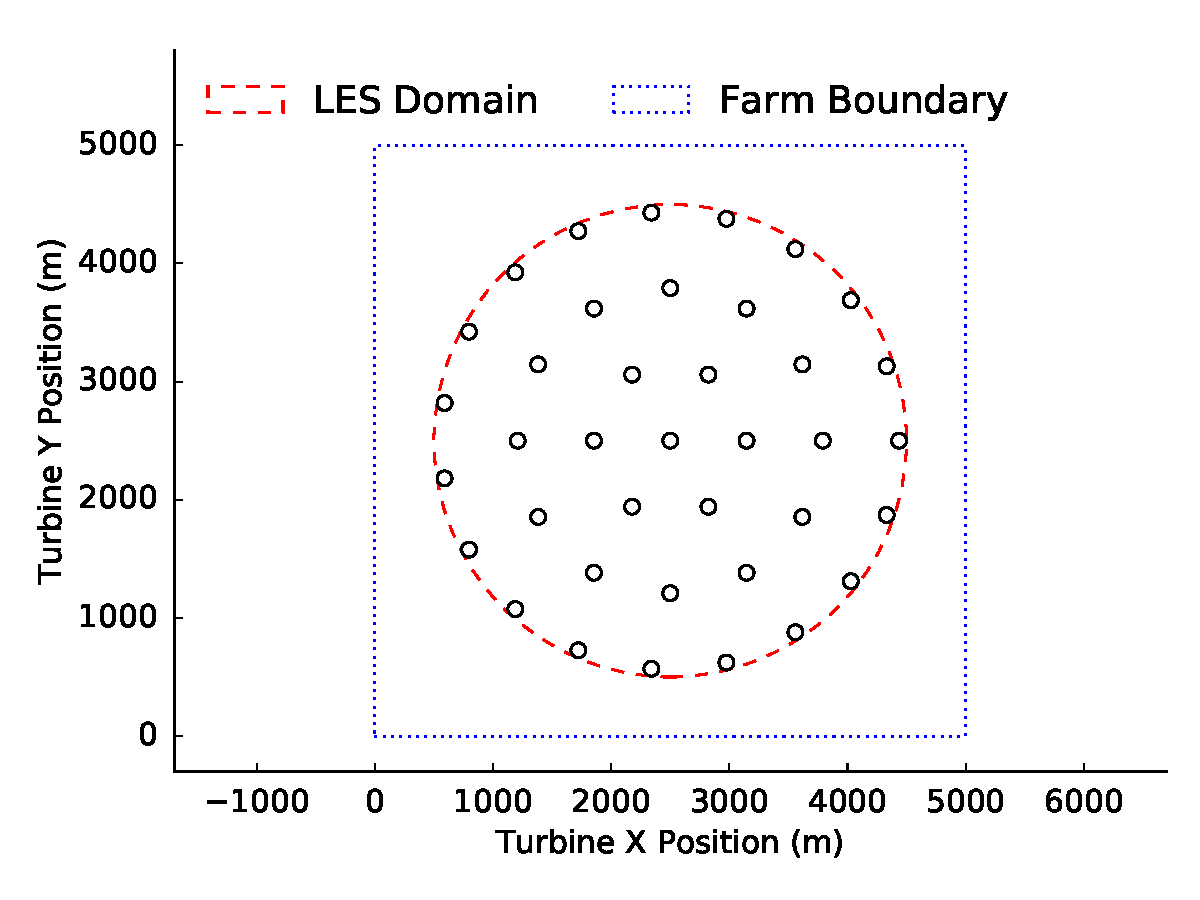
\includegraphics[width=0.75\textwidth]{final_images/round_farm_38Turbines_5DSpacing_start.pdf}
	\caption{Base case wind farm layout. The circles marking turbine locations are to scale, with diameters equal to the rotor diameter.}
	\label{fig:starting-layout}
\end{figure}

For the wind frequencies, we chose to use the Nantucket wind rose \cite{wrcc2017}. %was selected as an approximation of the wind rose of the new Bay State Wind farm proposed for development off the coast of Massachusetts \cite{baystate2017}
To reduce the computational cost of the LES simulations, we generated a wind rose with 12 directions by binning every 3 directions from the Nantucket wind rose starting with wind from the north. We used the 12-direction wind rose for both the optimizations and the LES. The original and final wind roses are shown in \Cref{fig:windrose}.

\begin{figure}[ht]
	\centering
	\subfigure[]{
		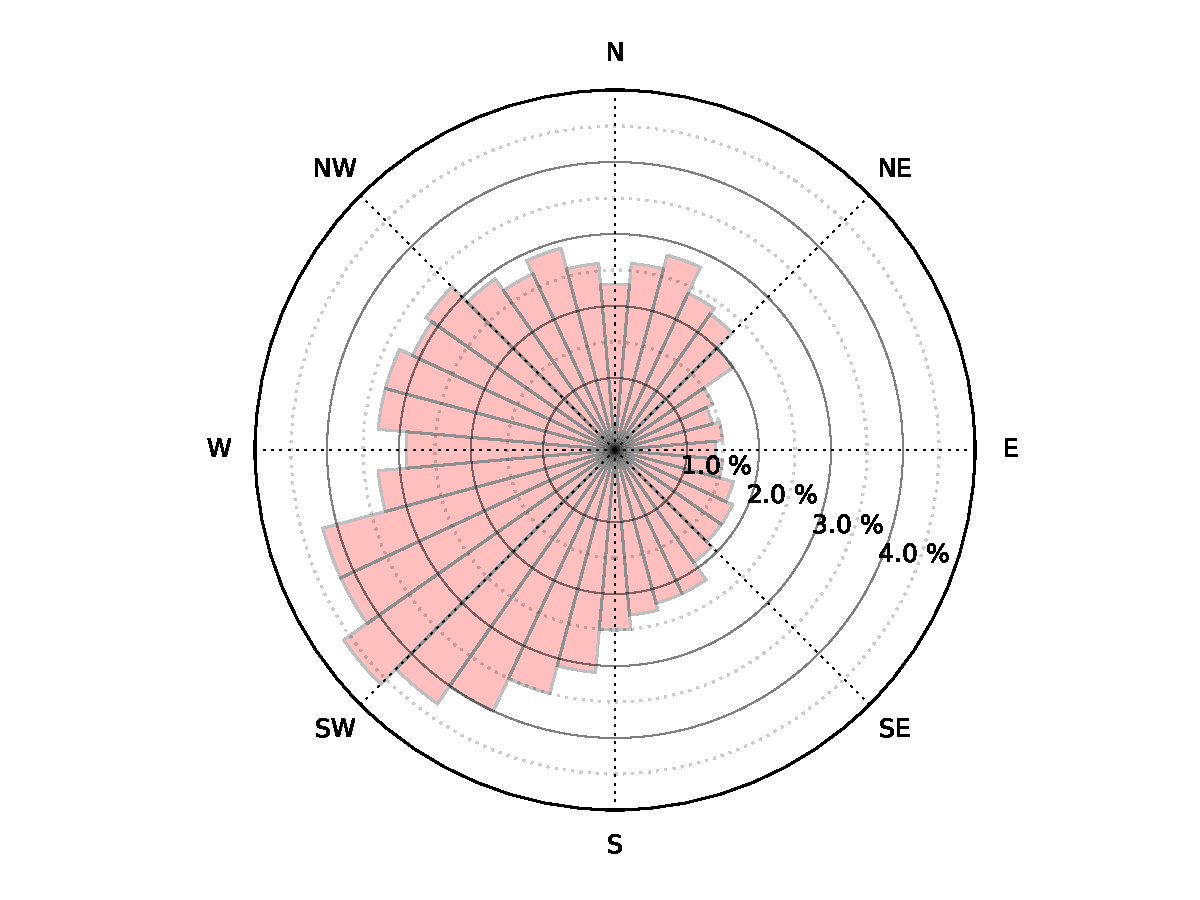
\includegraphics[width=0.48\textwidth, trim={3.25cm 0cm 3.25cm 0cm}]{final_images/windrose_full.pdf}
	}
	\subfigure[]{
		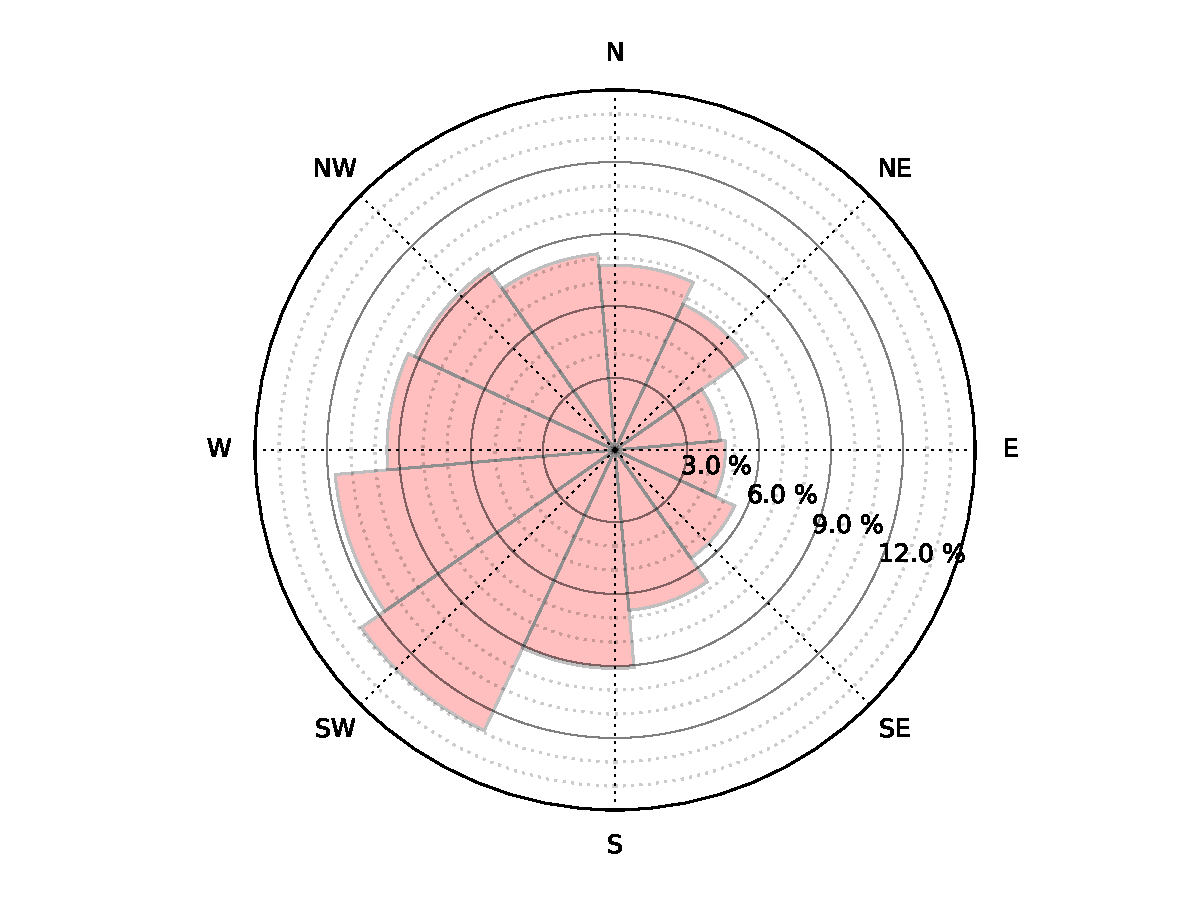
\includegraphics[width=0.48\textwidth, trim={3.25cm 0cm 3.25cm 0cm}]{final_images/windrose_les.pdf}
	}
	\caption{(a) Nantucket frequency wind rose \cite{wrcc2017}. (b) Nantucket frequency wind rose binned into 12 directions}
	\label{fig:windrose}
\end{figure}

\subsection{Optimization}\label{sec:opt}

We optimized the wind farm layout using AEP as the objective. The optimization problem was formulated as shown in \Cref{eq:objective}.
%
\begin{equation}
	\label{eq:objective}
	\begin{aligned} [b]
	\underset{x_i,y_i}{\textrm{maximize}} \quad & AEP(x_i,y_i,)~~i=1...38\\
	\textrm{subject to} \quad & S_{ij} \geq 2\*d~~i,j=1...38~~i \neq j\\
	 & [x_c-x_i]^2+[y_c-y_i]^2 \leq r_{b}^2~~i=1...38\\
	\end{aligned}
\end{equation}
%
In \Cref{eq:objective}, $(x_i,y_i)$ is the position of each turbine $i$, $S_{ij}$ represents the separation distance between each pair of turbines $i$ and $j$, $(x_c,y_c)$ is the location of the center of the wind farm, and $r_b$ is the radius of the wind farm boundary.

The optimization problem was built in OpenMDAO, a Multidisciplinary Design Analysis and Optimization platform  \cite{gray2010_OpenMDAO}. Gradients of the wake model were obtained using Tapenade, an algorithmic differentiation tool \cite{tapenade2013}. Gradients of all other system components were derived by hand. The final system gradients were compiled by OpenMDAO.

The gradients of both the objective function and constraints were scaled to be close to order one. The final problem was then solved using the Sparse Nonlinear OPTimizer (SNOPT), a gradient-based optimization algorithm that uses a sequential quadratic programming approach. SNOPT was used in this case because it is well suited to nonlinear problems with high dimensionality \cite{gill2005}. 

Along with SNOPT, we used the wake expansion continuation (WEC) method for reducing the multimodality of the wind farm layout optimization problem \cite{thomas2018-wec}. WEC relaxation factors ran from at $3.00$ down to, and including, $1.00$ in steps of $0.25$.  After completing the WEC series, we ran one final optimization, from the optimized layout found using WEC. In the final optimization, local turbulence intensity was calculated with the smooth maximum function as in \Cref{eq:smoothmax3}. For final wind farm assessment, we calculated local turbulence intensity using the hard maximum as done in \cite{niayifar2016}. 

As mentioned in \Cref{sec:ti}, we used three methods for calculating TI: (1) constant ambient TI only, (2) local TI calculated with a smooth max, and (3) local TI calculated with a hard maximum as done in the NP wind farm model. Because the hard maximum (3) creates discontinuities in the model and is not differentiable, we used a smooth maximum function (2) in the final step of our optimization process.  Calculating local TI as done in the NP wind farm model, with either the hard or smooth maximum functions, adds additional local optima that are exaggerated when using WEC. The additional local optima drastically reduce the effectiveness of the WEC method, so we neglected local turbulence intensity during the WEC optimization series. 

To arrive at the final optimized solution, we used a multistart optimization approach. Starting locations we used were the baseline layout shown in \Cref{fig:starting-layout}, as well as 199 pseudo-random layouts meeting the constraints of the optimization problem.

\subsection{Large-Eddy Simulation}

The simulator for wind farm applications (SOWFA) is a high-fidelity, large-eddy simulation tool that was developed at NREL for wind plant studies \cite{churchfieldnwtc,churchfield2012numerical,fleming2013sowfa}.  It is a computational fluid dynamics solver based on OpenFOAM \cite{jasak2007openfoam} and can model turbines as actuator disks or actuator lines.  This study uses turbines modeled as actuator disks to reduce computational cost.  Separate studies have been conducted that demonstrate that the steady-state power is similar in actuator disk and actuator line cases \cite{martinez2012comparison}.

SOWFA solves the three-dimensional, incompressible, Navier-Stokes equations and transport of potential temperature equations, which take into account the thermal buoyancy and Earth rotation (Coriolis) effects in the atmosphere.  The inflow conditions for these simulations are generated using a periodic atmospheric boundary layer precursor with no turbines.  

SOWFA calculates the unsteady flow field to compute the time-varying power, velocity deficits, and aerodynamic loads at each turbine in a wind plant.  This level of computation, with high-fidelity accuracy, takes on the order of hours to days to run on a supercomputer using a few hundred to a few thousand processors, depending on the size of the wind plant. The simulations run for this study were performed on Peregrine, NREL's high-performance computer \cite{regimbal2015peregrine}.

It should be noted that studies have been performed to validate SOWFA.  For example, it has been compared with 48-turbine Lillgrund wind plant field data and shows good agreement through the first five turbines in a row aligned with the wind direction \cite{churchfield2012large}.  In addition, SOWFA has been tested to verify that it captures the inertial range in the turbulent energy spectra and log-layer in the mean flow, both of which characterize a real atmospheric boundary layer \cite{churchfield2012numerical}.  Further validation studies are ongoing.  

Actuator disk simulations of the 38-turbine layout described in \Cref{sec:testcase}, as well as the  optimized layout, were performed using SOWFA.  To avoid needing a different precursor for each of  12 directions, the layout was rotated to a reference wind direction of 270$^\circ$.  The scenarios were simulated under neutral atmospheric conditions with an 8\,m/s mean wind speed at 80 m and approximately 10.8$\%$ turbulence intensity at hub height.

The simulations each ran for approximately 2000\,s of simulated time.  A structured mesh was used in this study with a grid spacing of 10\,m in the $x$, $y$, and $z$ directions resulting in a grid that is 500 $\times$ 500 $\times$ 100, i.e. 25,000,000 grid cells.  Using 500 cores, simulations took on the order of 1 day to complete.  

% \subsection{Comparing LES and Model Results}
% Comparison Approach

% Directional Power

% AEP

\section{Results and Discussion}

Due to the multimodal nature of the wind farm layout optimization problem, optimizing with the 200 different starting layouts resulted in a range of AEP values. While the optimizations were performed using 1 sample on the rotor-swept area, we used 100 samples across the rotor-swept area for the analysis. The distributions of AEP values as calculated with 1 and 100 samples across the rotor-swept area are shown in \cref{fig:opt-distribution}. Note that the distribution of AEP results is shifted lower when calculated using 100 samples on the rotor-swept area due to the denser sampling accounting for more wake effects. The next step was to determine the best layout. Calculating with 100 samples or 1 sample both indicate that the best layout is the one that started from the base case layout (shown in \cref{fig:starting-layout}). The final optimized layout is shown in \cref{fig:optimized-layout}.
%
\begin{figure}[htpb!]
	\centering
	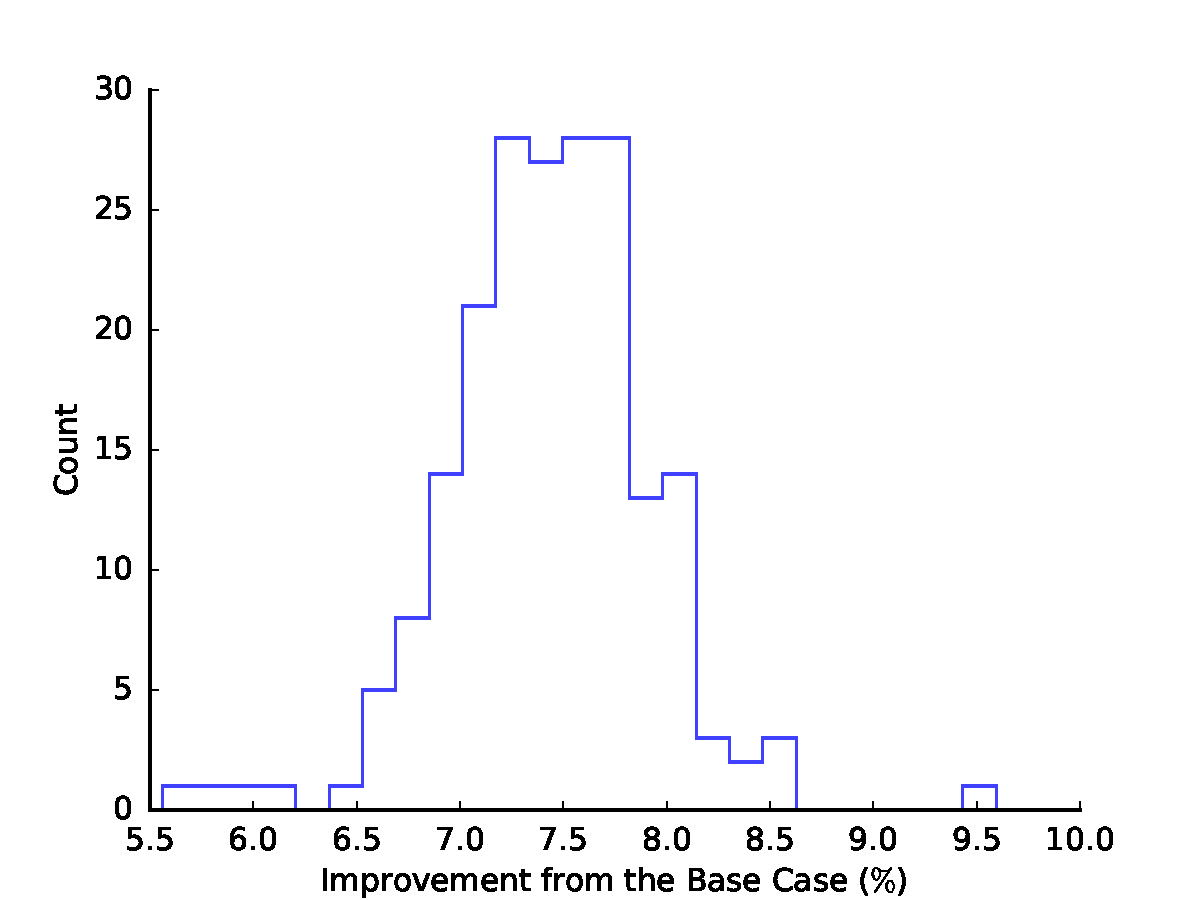
\includegraphics[width=0.75\textwidth]{final_images/38turbs_results_hist_aep.pdf}
	\caption{Distribution of AEP improvement calculated with 1 rotor sample point (black) and 100 rotor sample points (blue) from the 200 optimization runs. The high outlier started from the baseline layout. Note that the optimizations were performed using only 1 rotor sample point.}
	\label{fig:opt-distribution}
\end{figure}
%
\begin{figure}[htpb!]
	\centering
	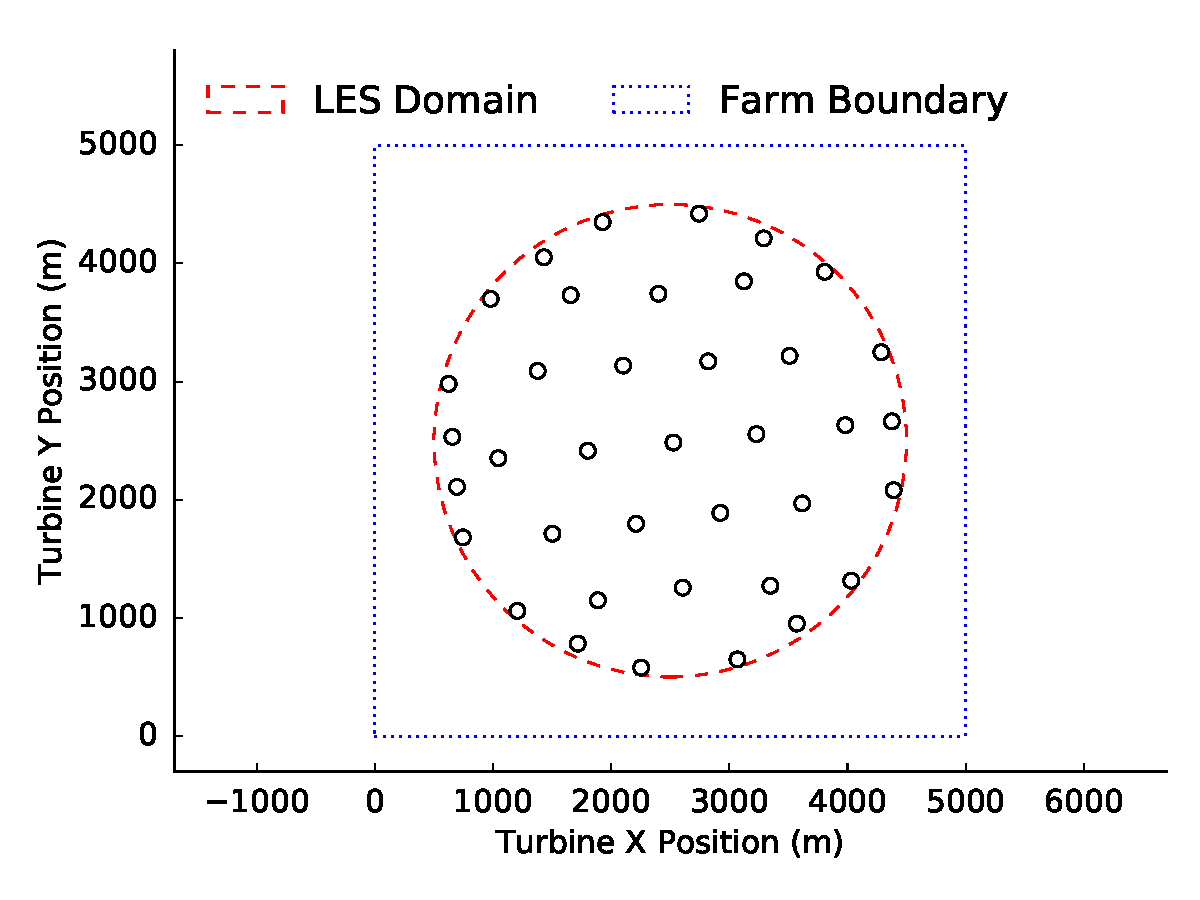
\includegraphics[width=0.75\textwidth]{final_images/round_farm_38Turbines_5DSpacing_finish.pdf}
	\caption{Optimized wind farm layout. The circles marking turbine locations are to scale, with diameters equal to the rotor diameter.}
	\label{fig:optimized-layout}
\end{figure}

We will now investigate the error with more granularity. The directional power production for both SOWFA and the BP model are shown in \cref{fig:dir-power}. The optimized power production in each direction for the optimized layout was nearly equal according to BP, with a spread of only \SI[per-mode=symbol]{0.3}{\mega\watt} across all directions. More variance appeared in the SOWFA results, which had a spread of \SI[per-mode=symbol]{3.4}{\mega\watt} across all directions for the optimized layout. The SOWFA predictions for the base case directions had more variation than BP as well. When we dive a little deeper we find the directional power predictions had errors ranging from $-5.4\%$ to $5.0\%$ for the base case layout and $-4.5\%$ to $0.8\%$ for the optimized layout, so some of the AEP improvement discrepancy is coming from the BP model underestimating the directional powers more for the optimized layout than the base case layout. The directional power errors for the base case layout have generally larger magnitudes than the directional errors for the optimized layout, but the directional errors for the base case layout are more equally distributed in the positive and negative than the directional errors for the optimized layout. Despite the directional errors, both the BP model and SOWFA predicted increased power production for every direction for the optimized layout as compared to the base case layout. The directional power, AEP, AEP improvement, and corresponding errors are reported in \cref{tab:validation-error}.
%
\begin{figure}[ht]
	\centering
	\subfigure[]{
		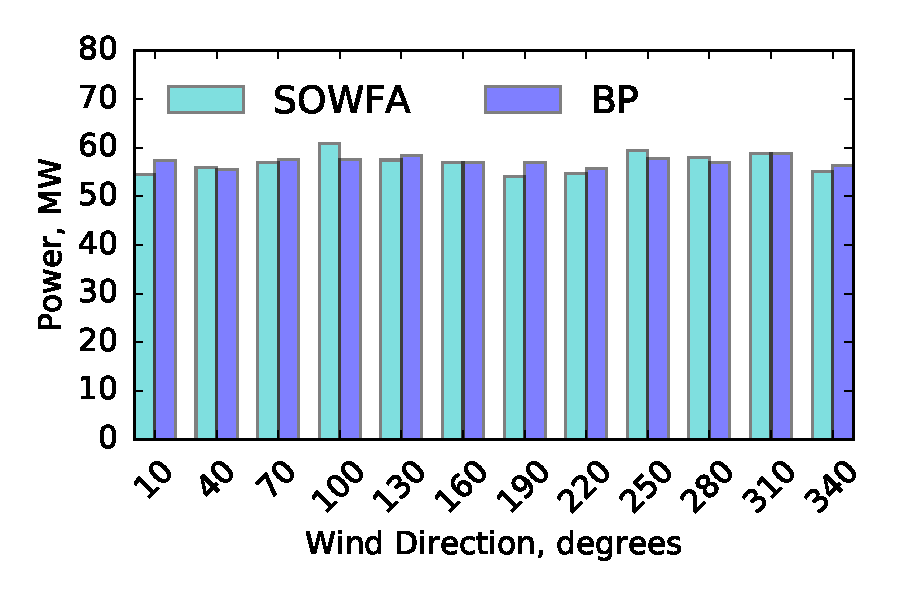
\includegraphics[width=0.48\textwidth, trim={0cm 0cm 0cm 0cm}]{final_images/sowfa_compare_pow_by_dir_base.pdf}
	}
	\subfigure[]{
		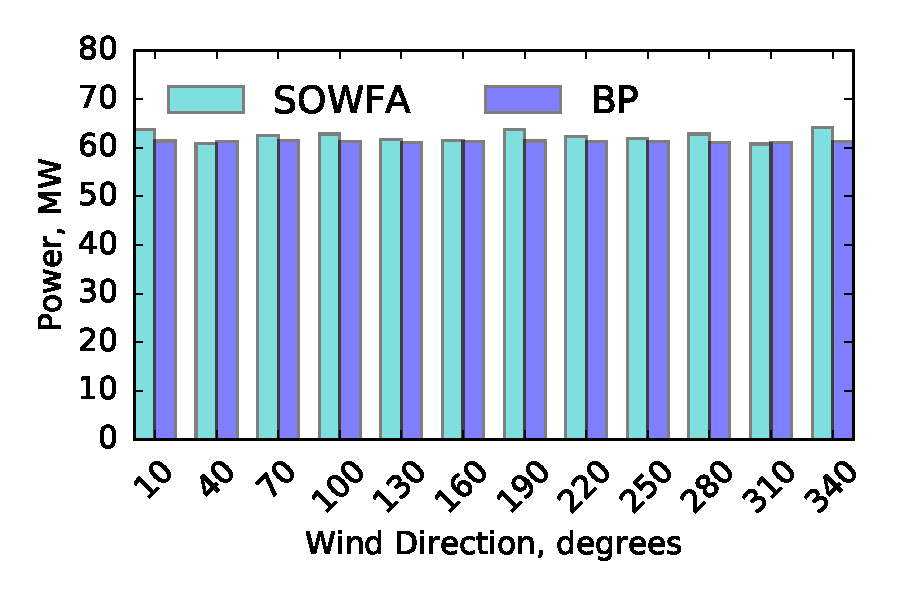
\includegraphics[width=0.48\textwidth, trim={0cm 0cm 0cm 0cm}]{final_images/sowfa_compare_pow_by_dir_opt.pdf}
	}
	\caption{Power production in each direction for SOWFA and the BP wake model using the hard maximum and 100 samples across the rotor for (a) the base layout (\Cref{fig:starting-layout}) and (b) the optimized layout (\Cref{fig:optimized-layout}).}
	\label{fig:dir-power}
\end{figure}

\begin{table*}[htpb!]\centering
\caption{BP and SOWFA Results}\label{tab:opt-results}
\ra{1.3}
\begin{tabular}{@{}lcrrrcrrrcrr@{}}\toprule
& \phantom{a} &\multicolumn{3}{c}{Base Case} &\phantom{a}& \multicolumn{3}{c}{Optimized} &\phantom{a}& \multicolumn{2}{c}{Improvement}\\ 
\cmidrule{3-5} \cmidrule{7-9} \cmidrule{11-12}

\multicolumn{1}{l}{Dir.} & \phantom{a} & \multicolumn{1}{c}{SOWFA} & \multicolumn{1}{c}{BP} & \multicolumn{1}{c}{Error} & \phantom{a} & \multicolumn{1}{c}{SOWFA} & \multicolumn{1}{c}{BP} & \multicolumn{1}{c}{Error} & \phantom{a} & \multicolumn{1}{c}{SOWFA} & \multicolumn{1}{c}{BP} \\ 
\cmidrule{1-1} \cmidrule{3-5} \cmidrule{7-9} \cmidrule{11-12}

%for dir: 10
%sowfa dir pow base, MW 54.5755549375
%sowfa dir pow opt, MW 63.6788126875
%bp dir pow base, MW 57.2975053819
%bp dir pow opt, MW 61.3969619942
%dir error base 0.049874901823
%dir error opt -0.0358337506151
%dir improvment sowfa 0.166801011193
%dir improvment bp 0.0715468602851

\multicolumn{1}{l}{$10^{\circ}$} & & \SI[per-mode=symbol]{54.6}{\mega\watt} &\SI[per-mode=symbol]{57.3}{\mega\watt} &\SI[per-mode=symbol]{5.0}{\percent} & &\SI[per-mode=symbol]{63.7}{\mega\watt} &\SI[per-mode=symbol]{61.4}{\mega\watt} &\SI[per-mode=symbol]{-3.6}{\percent} & &\SI[per-mode=symbol]{16.7}{\percent} &\SI[per-mode=symbol]{7.2}{\percent} \\

%for dir: 40
%sowfa dir pow base, MW 56.018788625
%sowfa dir pow opt, MW 60.8891199375
%bp dir pow base, MW 55.5160751359
%bp dir pow opt, MW 61.3612327815
%dir error base -0.00897401570882
%dir error opt 0.00775364867338
%dir improvment sowfa 0.0869410323223
%dir improvment bp 0.10528766004

\multicolumn{1}{l}{$40^{\circ}$} & & \SI[per-mode=symbol]{56.0}{\mega\watt} &\SI[per-mode=symbol]{55.5}{\mega\watt} &\SI[per-mode=symbol]{-0.9}{\percent} & &\SI[per-mode=symbol]{60.9}{\mega\watt} &\SI[per-mode=symbol]{61.4}{\mega\watt} &\SI[per-mode=symbol]{0.8}{\percent} & &\SI[per-mode=symbol]{8.7}{\percent} &\SI[per-mode=symbol]{10.5}{\percent} \\

%for dir: 70
%sowfa dir pow base, MW 56.9714324375
%sowfa dir pow opt, MW 62.5688415
%bp dir pow base, MW 57.5114463166
%bp dir pow opt, MW 61.4341340576
%dir error base 0.00947867827778
%dir error opt -0.0181353436509
%dir improvment sowfa 0.098249400147
%dir improvment bp 0.0682070786286

\multicolumn{1}{l}{$70^{\circ}$} & & \SI[per-mode=symbol]{57.0}{\mega\watt} &\SI[per-mode=symbol]{57.5}{\mega\watt} &\SI[per-mode=symbol]{0.9}{\percent} & &\SI[per-mode=symbol]{62.6}{\mega\watt} &\SI[per-mode=symbol]{61.4}{\mega\watt} &\SI[per-mode=symbol]{-1.8}{\percent} & &\SI[per-mode=symbol]{9.8}{\percent} &\SI[per-mode=symbol]{6.8}{\percent} \\

%for dir: 100
%sowfa dir pow base, MW 60.855835625
%sowfa dir pow opt, MW 62.831441
%bp dir pow base, MW 57.5595700861
%bp dir pow opt, MW 61.2262961942
%dir error base -0.0541651512138
%dir error opt -0.0255468405671
%dir improvment sowfa 0.032463696451
%dir improvment bp 0.063703153143

\multicolumn{1}{l}{$100^{\circ}$} & & \SI[per-mode=symbol]{60.9}{\mega\watt} &\SI[per-mode=symbol]{57.6}{\mega\watt} &\SI[per-mode=symbol]{-5.4}{\percent} & &\SI[per-mode=symbol]{62.8}{\mega\watt} &\SI[per-mode=symbol]{61.2}{\mega\watt} &\SI[per-mode=symbol]{-2.6}{\percent} & &\SI[per-mode=symbol]{3.2}{\percent} &\SI[per-mode=symbol]{6.4}{\percent} \\

%for dir: 130
%sowfa dir pow base, MW 57.493737
%sowfa dir pow opt, MW 61.6185440625
%bp dir pow base, MW 58.3991361881
%bp dir pow opt, MW 61.1745577966
%dir error base 0.0157477881126
%dir error opt -0.00720540013874
%dir improvment sowfa 0.0717435894365
%dir improvment bp 0.0475250455683

\multicolumn{1}{l}{$130^{\circ}$} & & \SI[per-mode=symbol]{57.5}{\mega\watt} &\SI[per-mode=symbol]{58.4}{\mega\watt} &\SI[per-mode=symbol]{1.6}{\percent} & &\SI[per-mode=symbol]{61.6}{\mega\watt} &\SI[per-mode=symbol]{61.2}{\mega\watt} &\SI[per-mode=symbol]{-0.7}{\percent} & &\SI[per-mode=symbol]{7.2}{\percent} &\SI[per-mode=symbol]{4.8}{\percent} \\

%for dir: 160
%sowfa dir pow base, MW 56.9407494062
%sowfa dir pow opt, MW 61.5216024375
%bp dir pow base, MW 56.9338836297
%bp dir pow opt, MW 61.2128242171
%dir error base -0.000120577557852
%dir error opt -0.00501902109473
%dir improvment sowfa 0.080449468597
%dir improvment bp 0.0751563096445

\multicolumn{1}{l}{$160^{\circ}$} & & \SI[per-mode=symbol]{56.9}{\mega\watt} &\SI[per-mode=symbol]{56.9}{\mega\watt} &\SI[per-mode=symbol]{-0.0}{\percent} & &\SI[per-mode=symbol]{61.5}{\mega\watt} &\SI[per-mode=symbol]{61.2}{\mega\watt} &\SI[per-mode=symbol]{-0.5}{\percent} & &\SI[per-mode=symbol]{8.0}{\percent} &\SI[per-mode=symbol]{7.5}{\percent} \\

%for dir: 190
%sowfa dir pow base, MW 54.07068575
%sowfa dir pow opt, MW 63.74526175
%bp dir pow base, MW 56.9132046155
%bp dir pow opt, MW 61.3955359552
%dir error base 0.0525704238089
%dir error opt -0.0368611835648
%dir improvment sowfa 0.178924603337
%dir improvment bp 0.078757317744

\multicolumn{1}{l}{$190^{\circ}$} & & \SI[per-mode=symbol]{54.1}{\mega\watt} &\SI[per-mode=symbol]{56.9}{\mega\watt} &\SI[per-mode=symbol]{5.3}{\percent} & &\SI[per-mode=symbol]{63.7}{\mega\watt} &\SI[per-mode=symbol]{61.4}{\mega\watt} &\SI[per-mode=symbol]{-3.7}{\percent} & &\SI[per-mode=symbol]{17.9}{\percent} &\SI[per-mode=symbol]{7.9}{\percent} \\

%for dir: 220
%sowfa dir pow base, MW 54.7768599375
%sowfa dir pow opt, MW 62.311719375
%bp dir pow base, MW 55.7754901851
%bp dir pow opt, MW 61.3053475038
%dir error base 0.0182308779428
%dir error opt -0.0161506034711
%dir improvment sowfa 0.137555519723
%dir improvment bp 0.0991449344561

\multicolumn{1}{l}{$220^{\circ}$} & & \SI[per-mode=symbol]{54.8}{\mega\watt} &\SI[per-mode=symbol]{55.8}{\mega\watt} &\SI[per-mode=symbol]{1.8}{\percent} & &\SI[per-mode=symbol]{62.3}{\mega\watt} &\SI[per-mode=symbol]{61.3}{\mega\watt} &\SI[per-mode=symbol]{-1.6}{\percent} & &\SI[per-mode=symbol]{13.8}{\percent} &\SI[per-mode=symbol]{9.9}{\percent} \\

%for dir: 250
%sowfa dir pow base, MW 59.470990875
%sowfa dir pow opt, MW 61.88793425
%bp dir pow base, MW 57.7326222423
%bp dir pow opt, MW 61.3319085252
%dir error base -0.0292305308369
%dir error opt -0.00898439625615
%dir improvment sowfa 0.0406407113693
%dir improvment bp 0.0623440637736

\multicolumn{1}{l}{$250^{\circ}$} & & \SI[per-mode=symbol]{59.5}{\mega\watt} &\SI[per-mode=symbol]{57.7}{\mega\watt} &\SI[per-mode=symbol]{-2.9}{\percent} & &\SI[per-mode=symbol]{61.9}{\mega\watt} &\SI[per-mode=symbol]{61.3}{\mega\watt} &\SI[per-mode=symbol]{-0.9}{\percent} & &\SI[per-mode=symbol]{4.1}{\percent} &\SI[per-mode=symbol]{6.2}{\percent} \\

%for dir: 280
%sowfa dir pow base, MW 57.936899875
%sowfa dir pow opt, MW 62.844579375
%bp dir pow base, MW 56.8889908634
%bp dir pow opt, MW 61.1815554536
%dir error base -0.0180870742808
%dir error opt -0.0264624879012
%dir improvment sowfa 0.0847073196976
%dir improvment bp 0.0754551016836

\multicolumn{1}{l}{$280^{\circ}$} & & \SI[per-mode=symbol]{57.9}{\mega\watt} &\SI[per-mode=symbol]{56.9}{\mega\watt} &\SI[per-mode=symbol]{-1.8}{\percent} & &\SI[per-mode=symbol]{62.8}{\mega\watt} &\SI[per-mode=symbol]{61.2}{\mega\watt} &\SI[per-mode=symbol]{-2.6}{\percent} & &\SI[per-mode=symbol]{8.5}{\percent} &\SI[per-mode=symbol]{7.5}{\percent} \\

%for dir: 310
%sowfa dir pow base, MW 58.849970625
%sowfa dir pow opt, MW 60.786135875
%bp dir pow base, MW 58.8073143596
%bp dir pow opt, MW 61.0781349831
%dir error base -0.00072483070066
%dir error opt 0.00480371229235
%dir improvment sowfa 0.0329000206701
%dir improvment bp 0.0386145949408

\multicolumn{1}{l}{$310^{\circ}$} & & \SI[per-mode=symbol]{58.8}{\mega\watt} &\SI[per-mode=symbol]{58.8}{\mega\watt} &\SI[per-mode=symbol]{-0.1}{\percent} & &\SI[per-mode=symbol]{60.8}{\mega\watt} &\SI[per-mode=symbol]{61.1}{\mega\watt} &\SI[per-mode=symbol]{.5}{\percent} & &\SI[per-mode=symbol]{3.3}{\percent} &\SI[per-mode=symbol]{3.9}{\percent} \\

%for dir: 340
%sowfa dir pow base, MW 55.0902787812
%sowfa dir pow opt, MW 64.1653636875
%bp dir pow base, MW 56.427558609
%bp dir pow opt, MW 61.2709414163
%dir error base 0.0242743340089
%dir error opt -0.0451087955382
%dir improvment sowfa 0.164731148707
%dir improvment bp 0.0858336409841
\multicolumn{1}{l}{$340^{\circ}$} & & \SI[per-mode=symbol]{55.1}{\mega\watt} &\SI[per-mode=symbol]{56.4}{\mega\watt} &\SI[per-mode=symbol]{2.4}{\percent} & &\SI[per-mode=symbol]{64.2}{\mega\watt} &\SI[per-mode=symbol]{61.3}{\mega\watt} &\SI[per-mode=symbol]{-4.5}{\percent} & &\SI[per-mode=symbol]{16.5}{\percent} &\SI[per-mode=symbol]{8.6}{\percent} \\

\hline
%sowfa aep base, GWh 478.464478387
%sowfa aep opt, GWh 525.960215588
%bp aep base, GWh 480.984400368
%bp aep opt, GWh 516.410850883
%aep error base 0.00526668560714
%aep error opt -0.0181560589976
\multicolumn{1}{l}{AEP}& &\SI[per-mode=symbol]{478}{\giga\watt\hour} &\SI[per-mode=symbol]{481}{\giga\watt\hour} &\SI[per-mode=symbol]{0.5}{\percent} & &\SI[per-mode=symbol]{526}{\giga\watt\hour} &\SI[per-mode=symbol]{516}{\giga\watt\hour} &\SI[per-mode=symbol]{-1.8}{\percent} & &\SI[per-mode=symbol]{9.9}{\percent} &\SI[per-mode=symbol]{7.4}{\percent}\\ 
%aep improvement sowfa 0.0992670079945
%aep improvement bp 0.0736540529952
 \bottomrule
\end{tabular}

\end{table*}
%

Just as the directional errors are larger than the AEP errors, the wind turbine power errors are, in general, much greater than the directional errors. Power production errors for individual turbines ranged from $-27.6\%$ to $96.6\%$ for the base case layout and $-32.9\%$ to $118.4\%$ for the optimized layout. The BP model accurately predicted the direction of the change in power for only $61.6\%$ of the wind turbines. Power predictions for individual wind turbines have too much error to be trusted individually. It may be argued that if we can't trust the individual wind turbine power predictions, then the wind farm layout optimization can't be trusted either since the optimizer moves the turbines to improve their power and therefor the power of the farm as a whole. However, despite the turbine errors, the BP model still allows the optimizer to reduce wake effects, which is the primary driver for increasing power production in a real wind farm. The errors for power production for each turbine in each wind direction are shown in the appendix in \cref{fig:optimized-power-error,fig:basecase-power-error}.

We have found that each time we average turbine powers to get directional power, or average directional power to calculate AEP, the error decreases. The maximum errors at each level are as follows: $118.4\%$ for wind turbine power, $5.4\%$ for directional power, and $1.8\%$ for AEP. This is as expected since we know from the law of large numbers that the more samples that are combined to get an averaged result, the more precise that result tends to be. Our directional power and AEP values are essentially scaled means of sets of the values from the population of wind turbines. For example, the average turbine power error for the base case and optimized layouts respectively are $5.6\%$ and $1.0\%$, with standard deviations of $21.6\%$ and $16.6\%$. We can then place some confidence in AEP and directional power predictions from the BP model. We have shown that the overall improvements in directional power for this case are not just a factor of the simplified wake model since the AEP improvement is shown to be even greater according to SOWFA simulations than predicted by the BP model.

\section{Conclusion}
In this work, we have made some adjustments to the 2016 Bastankhah and Port\'{e}-Agel wake model and the 2016 Niayifar and Port\'{e}-Agel wind farm model for improved compatibility with gradient-based optimization methods. We then demonstrated that our implementation of our altered models met or exceeded the accuracy of the models presented by Bastankhah, Niayifar, and Port\'{e}-Agel as compared to the LES data presented by Niayifar and Port\'{e}-Agel in \cite{niayifar2016}. We described our test case and gradient-based optimization methods, as well as the SOWFA set up used to produce the LES results that we used to check the model and optimization results. We found the individual turbine predictions based on the models had large errors as compared to our SOWFA simulations, up to $118.4\%$. The directional and AEP errors were much less, up to only $5.4\%$ and $1.8\%$ respectively. The models predicted an improvement in AEP of $7.4\%$, while SOWFA predicted that the AEP improvement should be $9.9\%$. Based on these results, we conclude that while the individual turbine power predictions may not be accurate, the improvements in directional power and AEP, at least for this case, can be trusted and are not simply an artifact of the simplified models being used during optimization.

Future work should include further analysis of the individual wind turbine power errors, an investigation of methods for sampling wind speeds across the rotor-swept area, and demonstration of optimization improvements in other wind farms and wind conditions using simulations. More wind tunnel tests of optimized wind farms are needed to validate the results of wind farm layout optimization using simplified models.

%The final layout with the highest AEP is shown in \Cref{fig:final-layout}.

% \begin{figure}[ht]
% 	\centering
% 	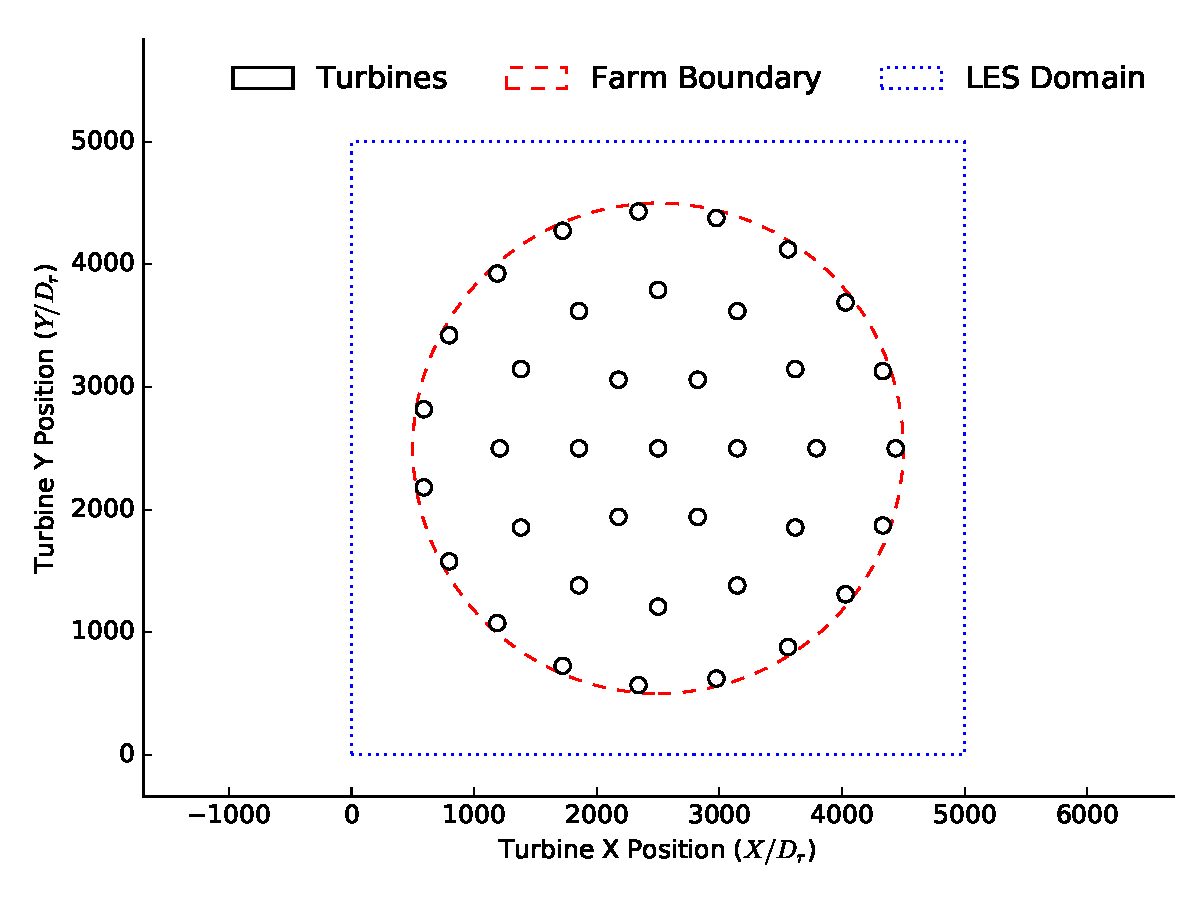
\includegraphics[width=0.75\textwidth]{final_images/round_farm_38Turbines_5DSpacing.pdf}
% 	\caption{Final optimized layout with the highest AEP. Obtained using the starting positions shown in \Cref{fig:starting-layout}}
% 	\label{fig:final-layout}
% \end{figure}

% \subsubsection{Simplified Modeling}

% \subsubsection{LES Modeling}

% \subsubsection{Comparison}

% \subsection{Expected Results}
% We will run the each of the 12 wind directions using LES for both the base layout and the final optimized layout. To validate the results, we will compare the percent improvement in: total AEP,  directional power for each direction, and the power production of each individual turbine in each direction. The optimization results will be considered validated if the relative change from base to optimized layout at each level of granularity (i.e. AEP, direction, and turbine) for LES and the Bastankhah and Port\'{e}-Agel wake model are similarly significant and follow similar trends. We may also be able to determine how much of the improvement is real. We plan to provide bar charts, results tables, and other figures as appropriate.

%cases you plan to run, how you plan to use LES, the metrics you will use to compare (and what would be considered ``validated''), etc.
% \section{Conclusion}
% This validation study will help us and other researchers understand how much of the improvement during optimization is real, and not an artifact of the models being used. This in turn will help us know how much improvement is needed based on simplified models to result in meaningful improvements to a real wind farm. 

\section*{Acknowledgments}

The authors developed this journal article based on funding from the Alliance for Sustainable Energy, LLC, Managing and Operating Contractor for the National Renewable Energy Laboratory for the U.S. Department of Energy. Funding for the work was provided by the DOE Office of Energy Efficiency and Renewable Energy, Wind Energy Technologies Office.

The U.S. Government retains and the publisher, by accepting the article for publication, acknowledges that the U.S. Government retains a nonexclusive, paid-up, irrevocable, worldwide license to publish or reproduce the published form of this work, or allow others to do so, for U.S. Government purposes.

A portion of the research was performed using computational resources sponsored by the Department of Energy's Office of Energy Efficiency and Renewable Energy and located at the National Renewable Energy Laboratory. 

A portion of the research was performed using computational resources of the Fulton Supercomputing Lab located at Brigham Young University.

\section*{Appendix}
The power production error for individual turbines in each direction for the 2016 Bastankhah and Port\'{e}-Agel wake model and the 2016 Niayifar and Port\'{e}-Agel wind farm model as compared to LES simulation performed using SOWFA are shown in \cref{fig:basecase-power-error}(a) and \cref{fig:optimized-power-error}(a). Directional power production errors for the models compared to the SOWFA results are shown in \cref{fig:basecase-power-error}(b) and \cref{fig:optimized-power-error}(b).
%
\begin{figure}[htpb!]
	\centering
	\subfigure[]{
		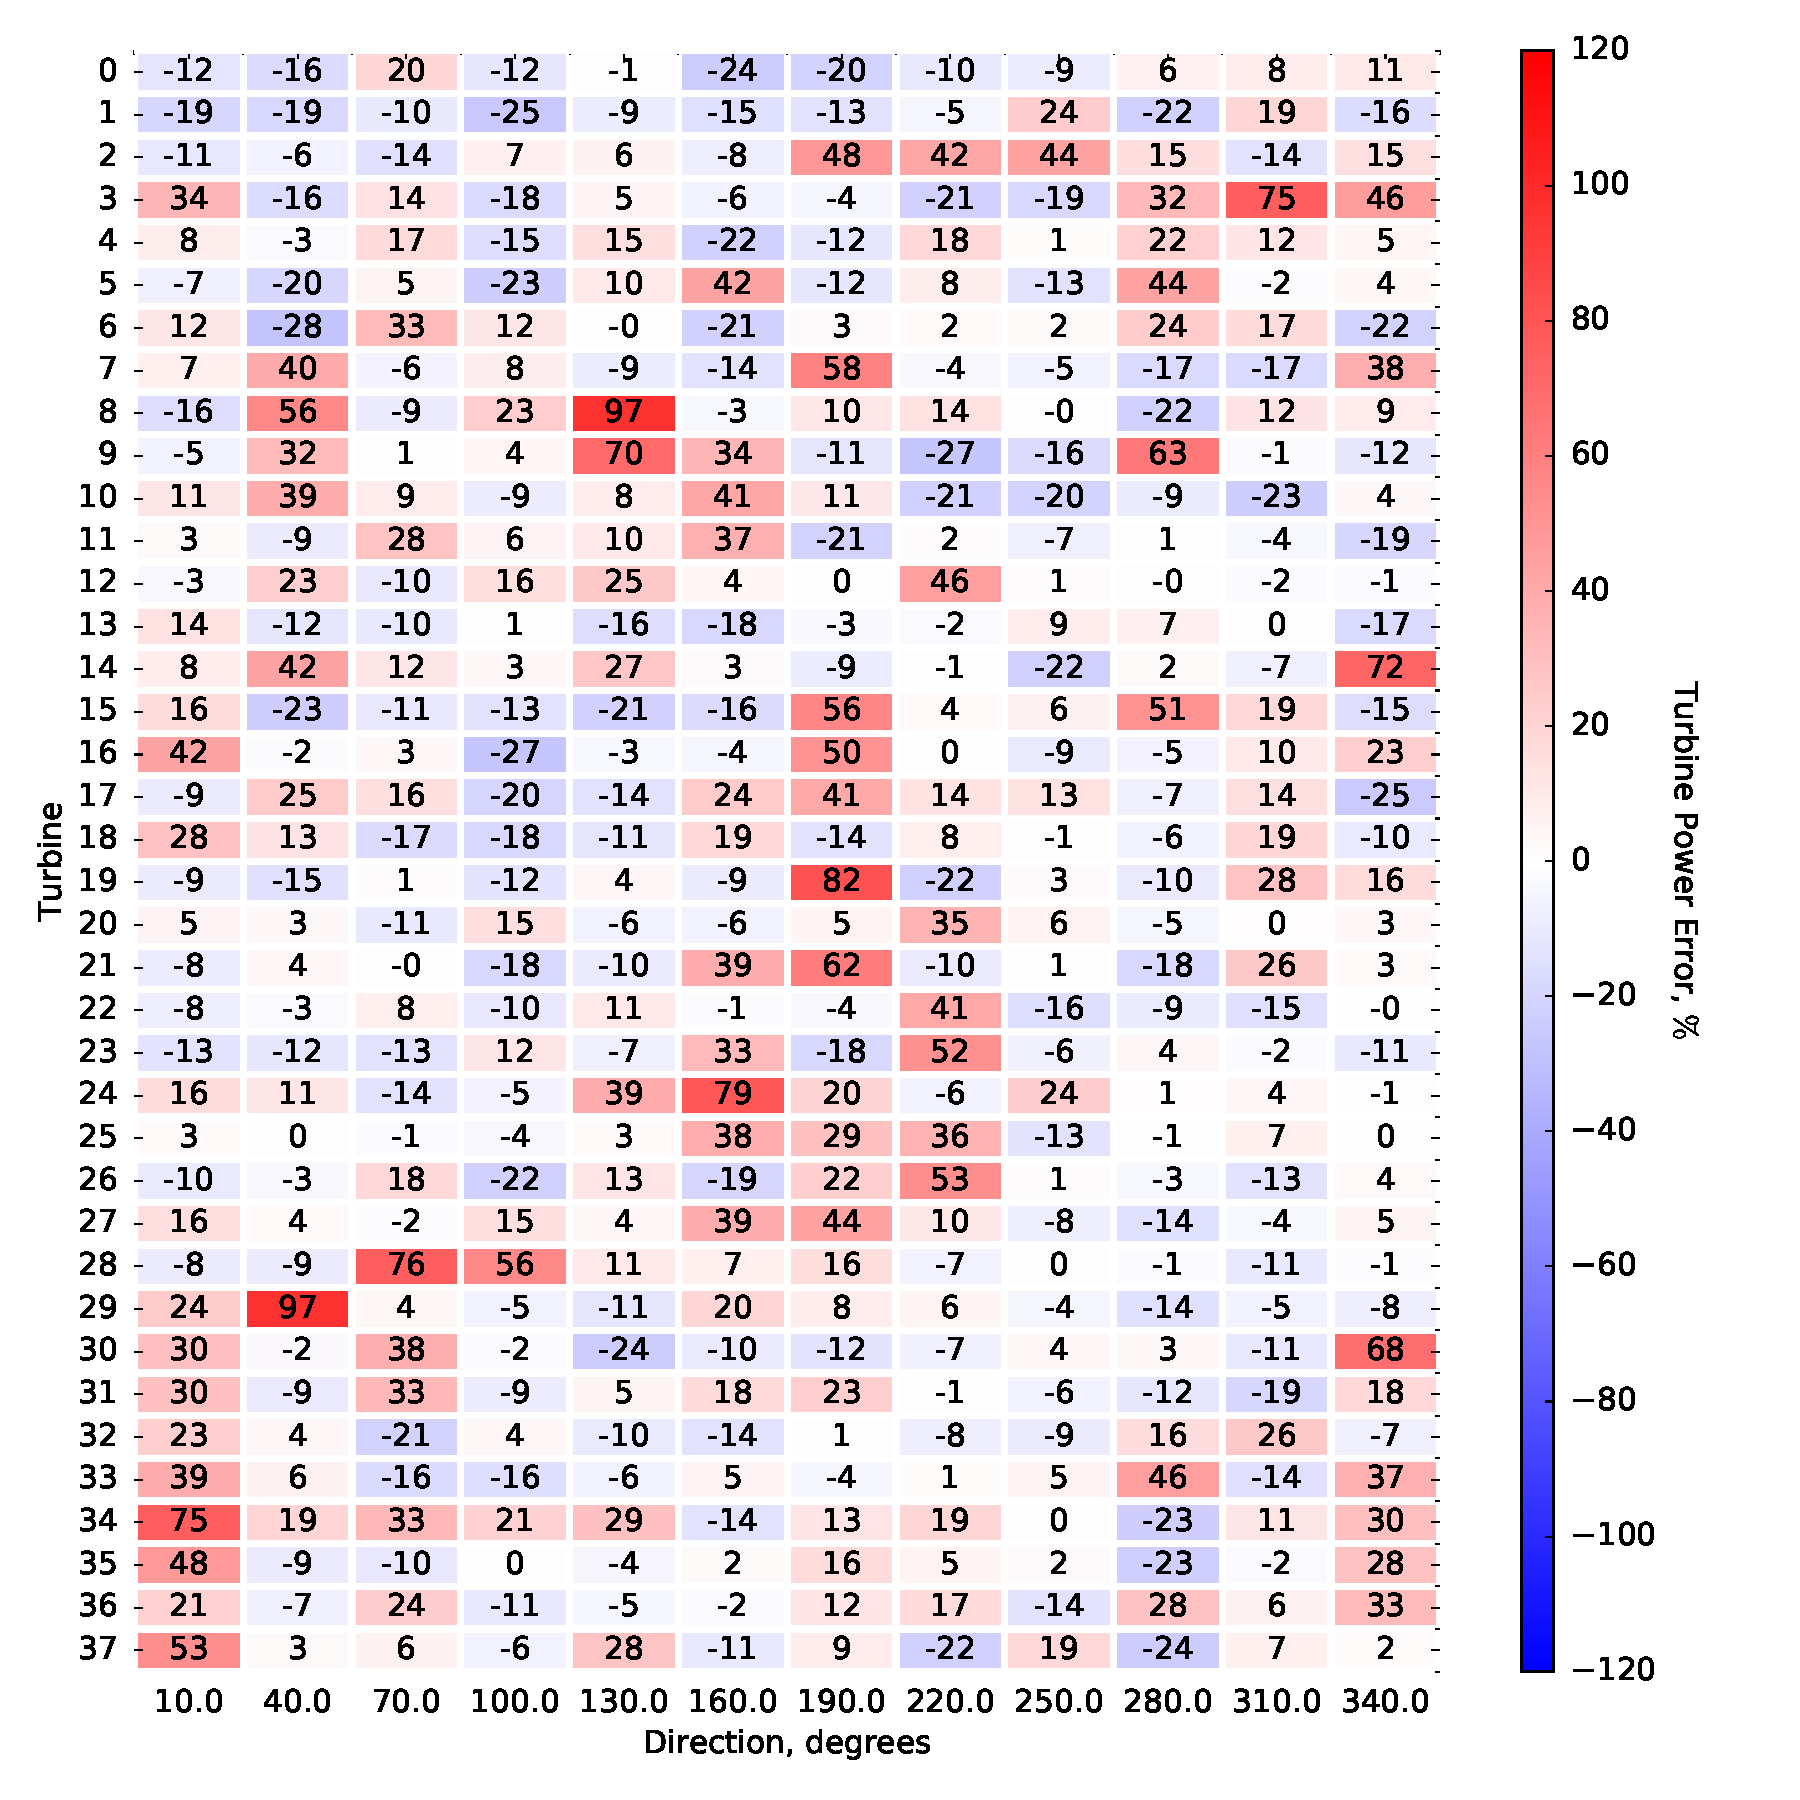
\includegraphics[width=0.98\textwidth, trim={0cm 0cm 0cm 0cm}]{final_images/sowfa_compare_pow_by_turb_dir_error_base.pdf}
	}
	\subfigure[]{
		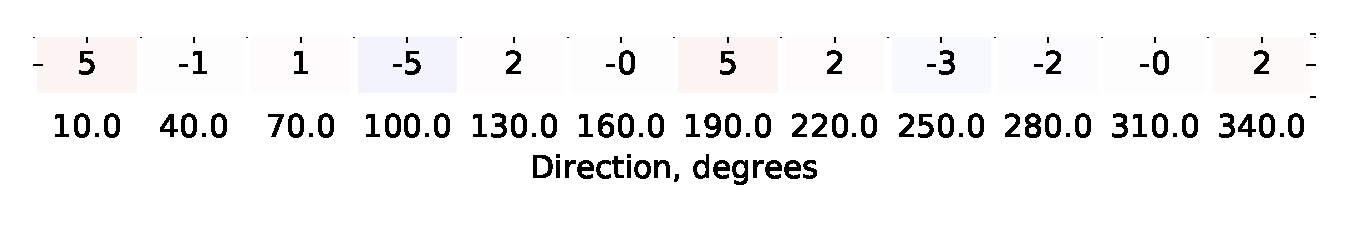
\includegraphics[width=0.77\textwidth, trim={1.75cm 0cm -1.75cm 0cm}]{final_images/sowfa_compare_pow_by_dir_error_base.pdf}
	}
	\caption{(a) Power production error of individual turbines in each direction as compared to SOWFA for the base case layout (\Cref{fig:starting-layout}). (b) Directional power production error as compared to SOWFA for the base case layout (\Cref{fig:starting-layout}).  The color bar applies to both (a) and (b).}
	\label{fig:basecase-power-error}
\end{figure}

\begin{figure}[htpb!]
	\centering
	\subfigure[]{
		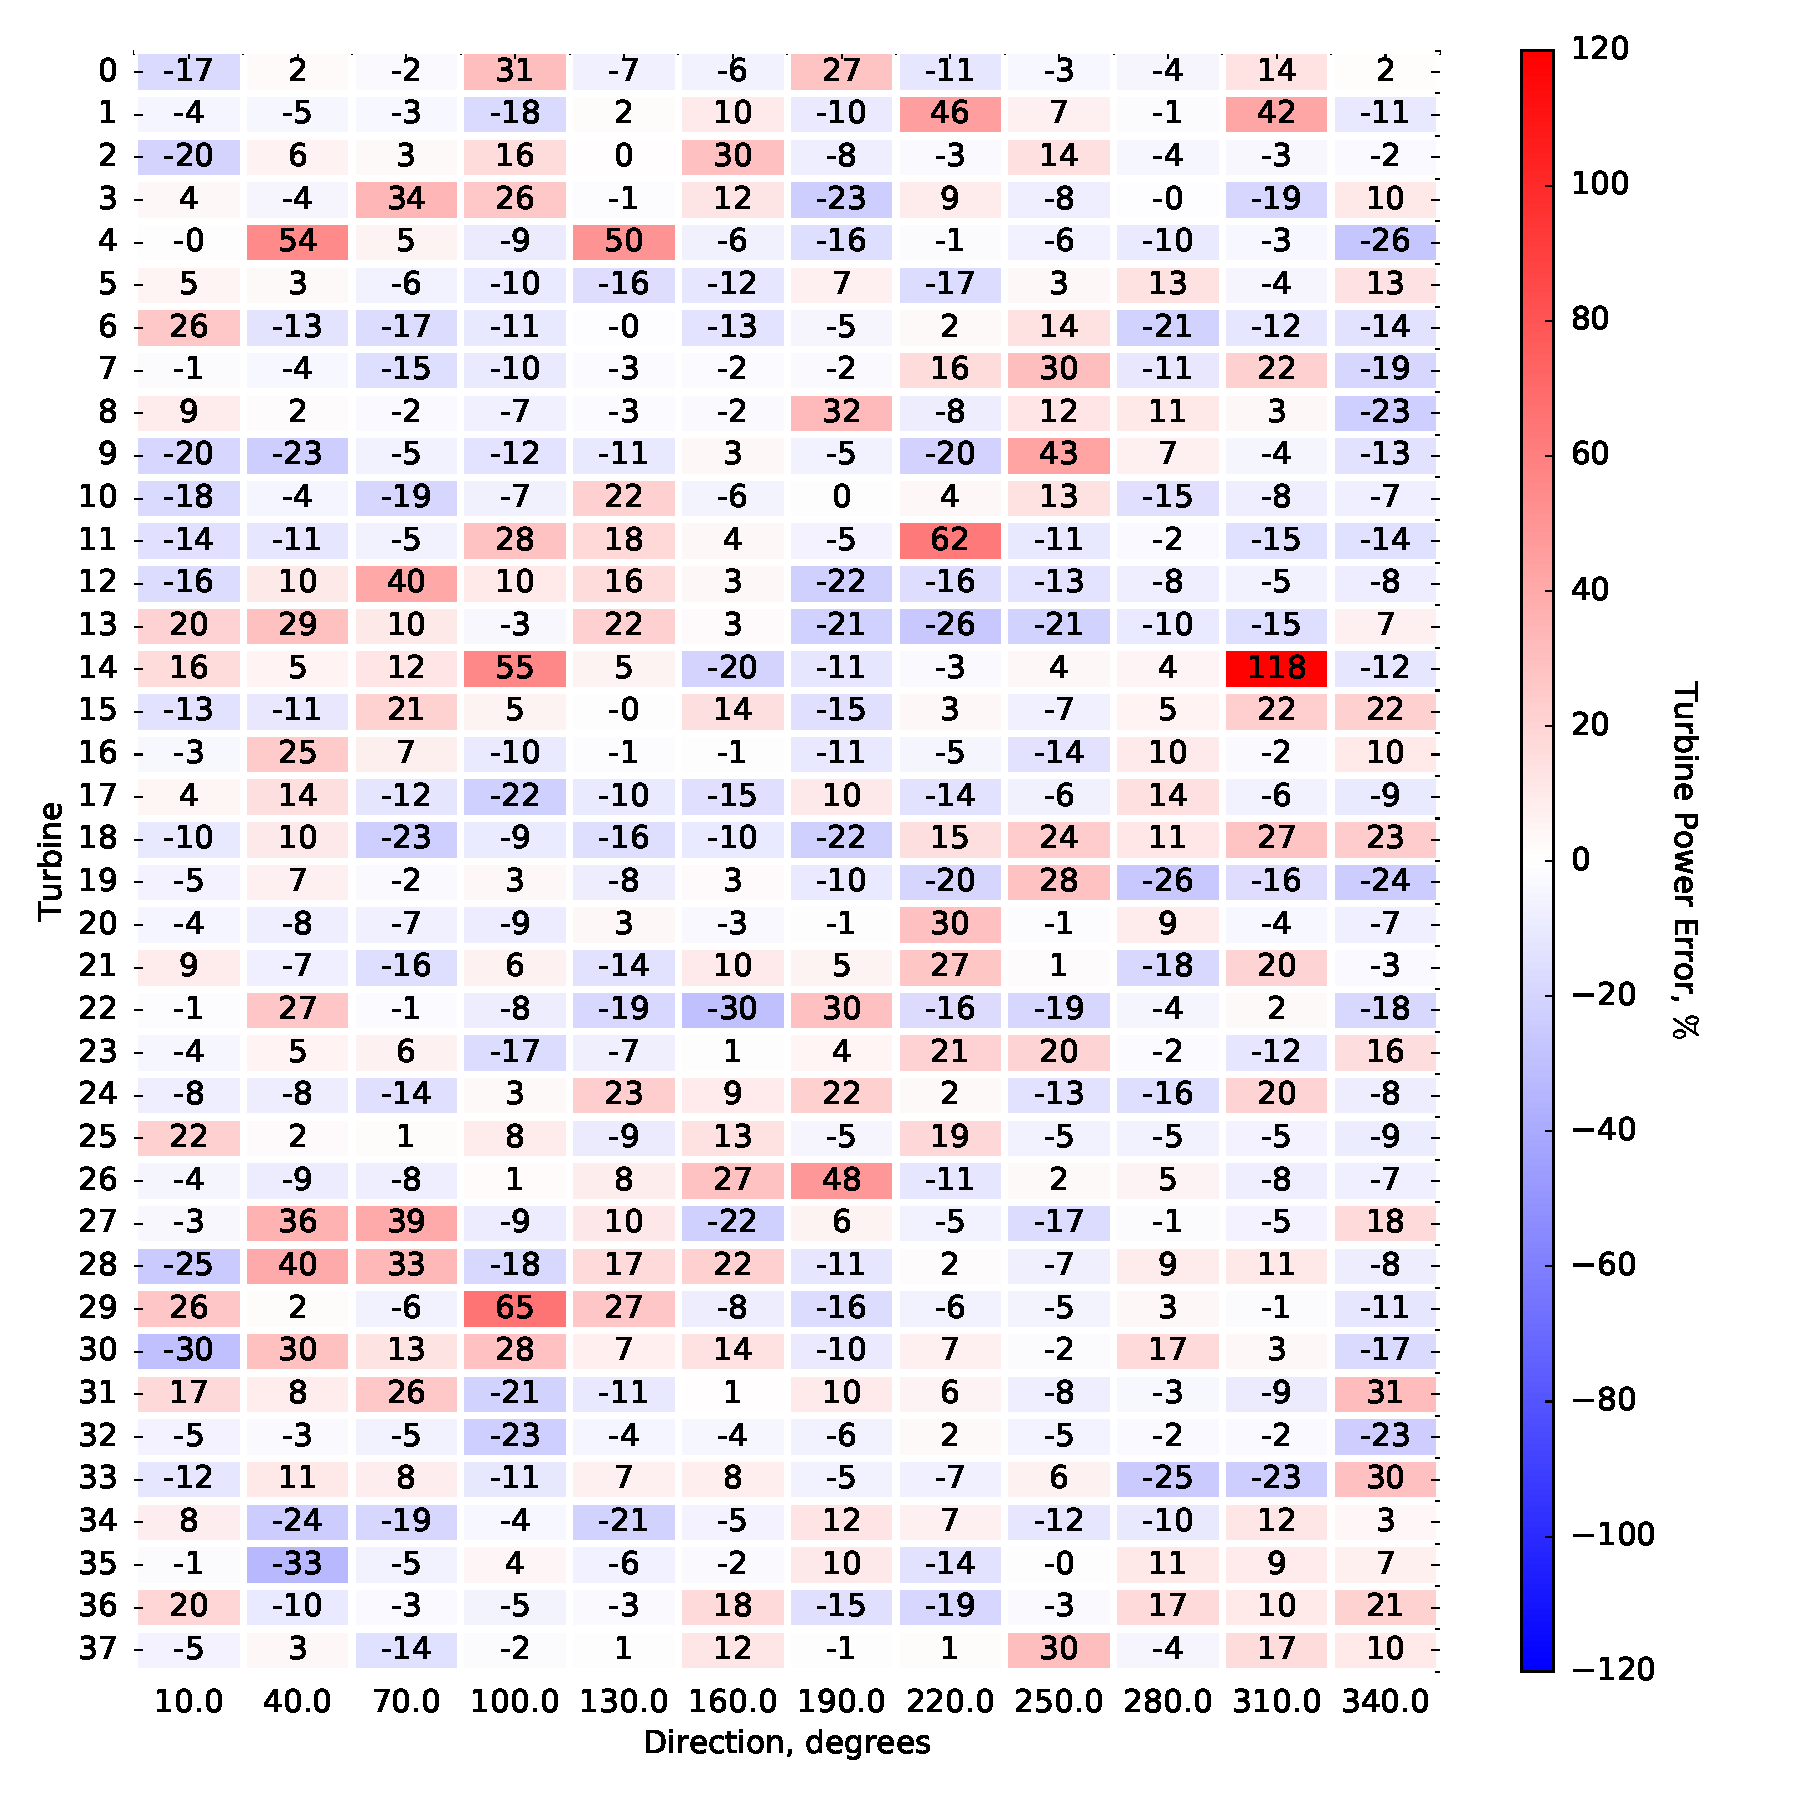
\includegraphics[width=0.98\textwidth, trim={0cm 0cm 0cm 0cm}]{final_images/sowfa_compare_pow_by_turb_dir_error_opt.pdf}
	}
	\subfigure[]{
		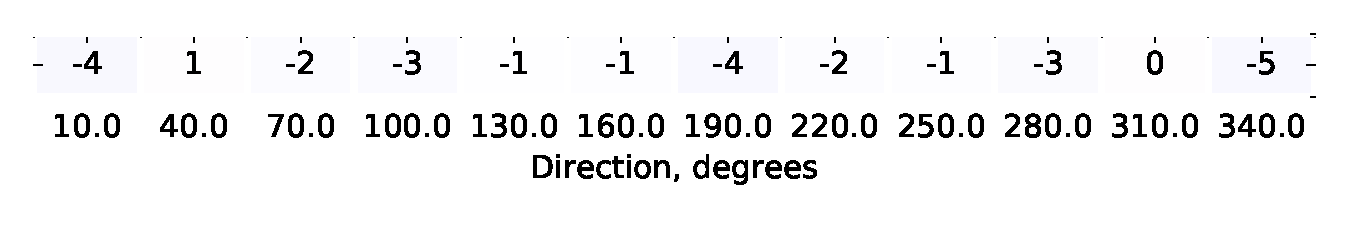
\includegraphics[width=0.77\textwidth, trim={1.75cm 0cm -1.75cm 0cm}]{final_images/sowfa_compare_pow_by_dir_error_opt.pdf}
	}
	\caption{(a) Power production error of individual turbines in each direction as compared to SOWFA for the optimized layout (\Cref{fig:optimized-layout}). (b) Directional power production error as compared to SOWFA for the optimized layout (\Cref{fig:optimized-layout}).  The color bar applies to both (a) and (b).}
	\label{fig:optimized-power-error}
\end{figure}

\clearpage 

\bibliographystyle{unsrt}
\bibliography{references/all_refs}
\end{document}